\documentclass[UTF8]{ctexart}
\usepackage[margin=2.2cm]{geometry}
\usepackage{tikz}
\usetikzlibrary{arrows.meta, positioning, fit}
\usepackage{graphicx}
\usepackage{float}
\floatplacement{figure}{H}
\floatplacement{table}{H}
\usepackage{amsmath}
\usepackage{booktabs}
\usepackage{longtable}
\usepackage{hyperref}

\title{ASIC 课程项目报告\\人体反应速率检测系统}
\author{田毓同\quad 23307110048}
\date{\today}

\begin{document}
\maketitle
\tableofcontents
\clearpage

\section{设计规划}

\subsection{设计要求}
本设计实现一个人体反应测试系统，主要要求如下：
\begin{enumerate}
  \item 使用四位八段数码管显示系统状态与测量结果。
  \item 使用 START 与 REACT 两个按键控制测试流程。
  \item START 后进入随机等待阶段，显示 \texttt{----}；随机等待结束后显示反应提示。
  \item 记录用户反应时间，分辨率为 1 ms；有效反应范围为 $100\,\mathrm{ms}\le t\le 5000\,\mathrm{ms}$。
  \item 过早按键或超出有效范围时显示 \texttt{Fail}。
  \item 支持显示最近三次有效成绩的平均值。
\end{enumerate}

\subsection{设计思路}
% 子文件用法：在主 tex 中加入 % 子文件用法：在主 tex 中加入 % 子文件用法：在主 tex 中加入 \input{report/section_2_2_design_idea.tex}
% 主 tex 导言区需要：\usepackage{tikz}
% 主 tex 导言区需要：\usetikzlibrary{arrows.meta, positioning}



本设计采用自顶向下的模块化设计方式，将 RTL 分为核心模块与外围交互模块两部分。核心模块负责状态转移、计时、历史记录和随机数生成等内部功能，并向外围显示模块提供数据与状态广播；外围模块接收核心状态并完成数码管显示、蜂鸣器提示，同时把按键控制输入经过去抖后反馈给核心模块。

测试流程由状态机统一调度。用户按下 START 键后，系统进入随机等待阶段，数码管显示等待提示；随机等待时间到达后，系统进入可反应阶段，数码管显示反应提示并启动反应时间计数。若用户在有效时间范围内按下 REACT 键，则系统记录并显示反应时间；若用户过早按键、反应时间小于最小阈值或超过最大阈值，则进入失败状态并显示 Fail。测试结束后再次按下 START 键显示最近三次有效成绩的平均值，再次按 START 开始下一轮测试。

随机等待时间由 LFSR 伪随机序列产生。为避免每次上电后完全固定、可预测的等待序列，随机模块在每次请求随机数时混入自由运行计数器的当前值。该计数器由系统时钟驱动，用户按下 START 的实际时刻会影响采样值，因此即使初始种子固定，每轮测试的等待时间也会受到人工按键时序扰动，从而降低可预测性。

% \subsubsection{反应测试状态机设计}

% 状态机包含 \texttt{IDLE}、\texttt{PREPARE}、\texttt{WAIT}、\texttt{REACT}、\texttt{FINISH}、\texttt{AVG} 和 \texttt{FAIL} 七个状态。状态转移关系如图~\ref{fig:reaction-fsm} 所示。

% \begin{figure}[htbp]
%   \centering
%   \begin{tikzpicture}[
%       >=Stealth,
%       node distance=20mm and 30mm,
%       state/.style={draw, rounded corners, minimum width=27mm, minimum height=10mm, align=center},
%       trans/.style={->, thick},
%       note/.style={font=\small, align=center}
%     ]

%     \node[state] (idle) {\texttt{IDLE}\\显示 0000};
%     \node[state, right=of idle] (prepare) {\texttt{PREPARE}\\请求随机数};
%     \node[state, right=of prepare] (wait) {\texttt{WAIT}\\显示 ----};
%     \node[state, below=of wait] (react) {\texttt{REACT}\\显示 $||||$};
%     \node[state, left=of react] (finish) {\texttt{FINISH}\\显示时间};
%     \node[state, below=of finish] (avg) {\texttt{AVG}\\显示平均值};
%     \node[state, below=of react] (fail) {\texttt{FAIL}\\显示 Fail};

%     \draw[trans] (idle) -- node[note, above] {START} (prepare);
%     \draw[trans] (prepare) -- node[note, above] {random\_valid\\锁存等待时间} (wait);
%     \draw[trans] (wait) -- node[note, right] {随机等待到达\\清零计数器} (react);
%     \draw[trans] (wait.east) -- ++(12mm,0) |- node[note, near start, right] {提前 REACT} (fail.east);

%     \draw[trans] (react) -- node[note, above] {有效 REACT\\$100\,\mathrm{ms}\le t\le5000\,\mathrm{ms}$} (finish);
%     \draw[trans] (react) -- node[note, right] {$t<100\,\mathrm{ms}$\\或 $t>5000\,\mathrm{ms}$} (fail);

%     \draw[trans] (finish) -- node[note, left] {START} (avg);
%     \draw[trans] (fail) -- node[note, below] {START} (avg);
%     \draw[trans] (avg.west) -- ++(-12mm,0) |- node[note, near start, left] {START\\下一轮} (prepare.west);

%   \end{tikzpicture}
%   \caption{反应测试系统状态机}
%   \label{fig:reaction-fsm}
% \end{figure}

% \begin{table}[htbp]
%   \centering
%   \caption{状态机状态说明}
%   \label{tab:reaction-fsm-state}
%   \begin{tabular}{c|l|l}
%     \hline
%     状态 & 显示内容 & 功能说明 \\
%     \hline
%     \texttt{IDLE} & \texttt{0000} & 空闲状态，等待 START 按键开始测试 \\
%     \texttt{PREPARE} & 保持上一显示 & 请求并锁存一组随机等待时间 \\
%     \texttt{WAIT} & \texttt{----} & 随机等待阶段，若提前按 REACT 则失败 \\
%     \texttt{REACT} & \texttt{$||||$} & 允许用户反应，计数器记录反应时间 \\
%     \texttt{FINISH} & 反应时间 & 有效反应结束，显示本次反应时间并写入历史记录 \\
%     \texttt{AVG} & 平均时间或 \texttt{0000} & 显示最近三次有效成绩平均值，无成绩时显示 \texttt{0000} \\
%     \texttt{FAIL} & \texttt{Fail} & 提前、过短或超时反应，等待 START 查看平均值 \\
%     \hline
%   \end{tabular}
% \end{table}

% 主 tex 导言区需要：\usepackage{tikz}
% 主 tex 导言区需要：\usetikzlibrary{arrows.meta, positioning}



本设计采用自顶向下的模块化设计方式，将 RTL 分为核心模块与外围交互模块两部分。核心模块负责状态转移、计时、历史记录和随机数生成等内部功能，并向外围显示模块提供数据与状态广播；外围模块接收核心状态并完成数码管显示、蜂鸣器提示，同时把按键控制输入经过去抖后反馈给核心模块。

测试流程由状态机统一调度。用户按下 START 键后，系统进入随机等待阶段，数码管显示等待提示；随机等待时间到达后，系统进入可反应阶段，数码管显示反应提示并启动反应时间计数。若用户在有效时间范围内按下 REACT 键，则系统记录并显示反应时间；若用户过早按键、反应时间小于最小阈值或超过最大阈值，则进入失败状态并显示 Fail。测试结束后再次按下 START 键显示最近三次有效成绩的平均值，再次按 START 开始下一轮测试。

随机等待时间由 LFSR 伪随机序列产生。为避免每次上电后完全固定、可预测的等待序列，随机模块在每次请求随机数时混入自由运行计数器的当前值。该计数器由系统时钟驱动，用户按下 START 的实际时刻会影响采样值，因此即使初始种子固定，每轮测试的等待时间也会受到人工按键时序扰动，从而降低可预测性。

% \subsubsection{反应测试状态机设计}

% 状态机包含 \texttt{IDLE}、\texttt{PREPARE}、\texttt{WAIT}、\texttt{REACT}、\texttt{FINISH}、\texttt{AVG} 和 \texttt{FAIL} 七个状态。状态转移关系如图~\ref{fig:reaction-fsm} 所示。

% \begin{figure}[htbp]
%   \centering
%   \begin{tikzpicture}[
%       >=Stealth,
%       node distance=20mm and 30mm,
%       state/.style={draw, rounded corners, minimum width=27mm, minimum height=10mm, align=center},
%       trans/.style={->, thick},
%       note/.style={font=\small, align=center}
%     ]

%     \node[state] (idle) {\texttt{IDLE}\\显示 0000};
%     \node[state, right=of idle] (prepare) {\texttt{PREPARE}\\请求随机数};
%     \node[state, right=of prepare] (wait) {\texttt{WAIT}\\显示 ----};
%     \node[state, below=of wait] (react) {\texttt{REACT}\\显示 $||||$};
%     \node[state, left=of react] (finish) {\texttt{FINISH}\\显示时间};
%     \node[state, below=of finish] (avg) {\texttt{AVG}\\显示平均值};
%     \node[state, below=of react] (fail) {\texttt{FAIL}\\显示 Fail};

%     \draw[trans] (idle) -- node[note, above] {START} (prepare);
%     \draw[trans] (prepare) -- node[note, above] {random\_valid\\锁存等待时间} (wait);
%     \draw[trans] (wait) -- node[note, right] {随机等待到达\\清零计数器} (react);
%     \draw[trans] (wait.east) -- ++(12mm,0) |- node[note, near start, right] {提前 REACT} (fail.east);

%     \draw[trans] (react) -- node[note, above] {有效 REACT\\$100\,\mathrm{ms}\le t\le5000\,\mathrm{ms}$} (finish);
%     \draw[trans] (react) -- node[note, right] {$t<100\,\mathrm{ms}$\\或 $t>5000\,\mathrm{ms}$} (fail);

%     \draw[trans] (finish) -- node[note, left] {START} (avg);
%     \draw[trans] (fail) -- node[note, below] {START} (avg);
%     \draw[trans] (avg.west) -- ++(-12mm,0) |- node[note, near start, left] {START\\下一轮} (prepare.west);

%   \end{tikzpicture}
%   \caption{反应测试系统状态机}
%   \label{fig:reaction-fsm}
% \end{figure}

% \begin{table}[htbp]
%   \centering
%   \caption{状态机状态说明}
%   \label{tab:reaction-fsm-state}
%   \begin{tabular}{c|l|l}
%     \hline
%     状态 & 显示内容 & 功能说明 \\
%     \hline
%     \texttt{IDLE} & \texttt{0000} & 空闲状态，等待 START 按键开始测试 \\
%     \texttt{PREPARE} & 保持上一显示 & 请求并锁存一组随机等待时间 \\
%     \texttt{WAIT} & \texttt{----} & 随机等待阶段，若提前按 REACT 则失败 \\
%     \texttt{REACT} & \texttt{$||||$} & 允许用户反应，计数器记录反应时间 \\
%     \texttt{FINISH} & 反应时间 & 有效反应结束，显示本次反应时间并写入历史记录 \\
%     \texttt{AVG} & 平均时间或 \texttt{0000} & 显示最近三次有效成绩平均值，无成绩时显示 \texttt{0000} \\
%     \texttt{FAIL} & \texttt{Fail} & 提前、过短或超时反应，等待 START 查看平均值 \\
%     \hline
%   \end{tabular}
% \end{table}

% 主 tex 导言区需要：\usepackage{tikz}
% 主 tex 导言区需要：\usetikzlibrary{arrows.meta, positioning}



本设计采用自顶向下的模块化设计方式，将 RTL 分为核心模块与外围交互模块两部分。核心模块负责状态转移、计时、历史记录和随机数生成等内部功能，并向外围显示模块提供数据与状态广播；外围模块接收核心状态并完成数码管显示、蜂鸣器提示，同时把按键控制输入经过去抖后反馈给核心模块。

测试流程由状态机统一调度。用户按下 START 键后，系统进入随机等待阶段，数码管显示等待提示；随机等待时间到达后，系统进入可反应阶段，数码管显示反应提示并启动反应时间计数。若用户在有效时间范围内按下 REACT 键，则系统记录并显示反应时间；若用户过早按键、反应时间小于最小阈值或超过最大阈值，则进入失败状态并显示 Fail。测试结束后再次按下 START 键显示最近三次有效成绩的平均值，再次按 START 开始下一轮测试。

随机等待时间由 LFSR 伪随机序列产生。为避免每次上电后完全固定、可预测的等待序列，随机模块在每次请求随机数时混入自由运行计数器的当前值。该计数器由系统时钟驱动，用户按下 START 的实际时刻会影响采样值，因此即使初始种子固定，每轮测试的等待时间也会受到人工按键时序扰动，从而降低可预测性。

% \subsubsection{反应测试状态机设计}

% 状态机包含 \texttt{IDLE}、\texttt{PREPARE}、\texttt{WAIT}、\texttt{REACT}、\texttt{FINISH}、\texttt{AVG} 和 \texttt{FAIL} 七个状态。状态转移关系如图~\ref{fig:reaction-fsm} 所示。

% \begin{figure}[htbp]
%   \centering
%   \begin{tikzpicture}[
%       >=Stealth,
%       node distance=20mm and 30mm,
%       state/.style={draw, rounded corners, minimum width=27mm, minimum height=10mm, align=center},
%       trans/.style={->, thick},
%       note/.style={font=\small, align=center}
%     ]

%     \node[state] (idle) {\texttt{IDLE}\\显示 0000};
%     \node[state, right=of idle] (prepare) {\texttt{PREPARE}\\请求随机数};
%     \node[state, right=of prepare] (wait) {\texttt{WAIT}\\显示 ----};
%     \node[state, below=of wait] (react) {\texttt{REACT}\\显示 $||||$};
%     \node[state, left=of react] (finish) {\texttt{FINISH}\\显示时间};
%     \node[state, below=of finish] (avg) {\texttt{AVG}\\显示平均值};
%     \node[state, below=of react] (fail) {\texttt{FAIL}\\显示 Fail};

%     \draw[trans] (idle) -- node[note, above] {START} (prepare);
%     \draw[trans] (prepare) -- node[note, above] {random\_valid\\锁存等待时间} (wait);
%     \draw[trans] (wait) -- node[note, right] {随机等待到达\\清零计数器} (react);
%     \draw[trans] (wait.east) -- ++(12mm,0) |- node[note, near start, right] {提前 REACT} (fail.east);

%     \draw[trans] (react) -- node[note, above] {有效 REACT\\$100\,\mathrm{ms}\le t\le5000\,\mathrm{ms}$} (finish);
%     \draw[trans] (react) -- node[note, right] {$t<100\,\mathrm{ms}$\\或 $t>5000\,\mathrm{ms}$} (fail);

%     \draw[trans] (finish) -- node[note, left] {START} (avg);
%     \draw[trans] (fail) -- node[note, below] {START} (avg);
%     \draw[trans] (avg.west) -- ++(-12mm,0) |- node[note, near start, left] {START\\下一轮} (prepare.west);

%   \end{tikzpicture}
%   \caption{反应测试系统状态机}
%   \label{fig:reaction-fsm}
% \end{figure}

% \begin{table}[htbp]
%   \centering
%   \caption{状态机状态说明}
%   \label{tab:reaction-fsm-state}
%   \begin{tabular}{c|l|l}
%     \hline
%     状态 & 显示内容 & 功能说明 \\
%     \hline
%     \texttt{IDLE} & \texttt{0000} & 空闲状态，等待 START 按键开始测试 \\
%     \texttt{PREPARE} & 保持上一显示 & 请求并锁存一组随机等待时间 \\
%     \texttt{WAIT} & \texttt{----} & 随机等待阶段，若提前按 REACT 则失败 \\
%     \texttt{REACT} & \texttt{$||||$} & 允许用户反应，计数器记录反应时间 \\
%     \texttt{FINISH} & 反应时间 & 有效反应结束，显示本次反应时间并写入历史记录 \\
%     \texttt{AVG} & 平均时间或 \texttt{0000} & 显示最近三次有效成绩平均值，无成绩时显示 \texttt{0000} \\
%     \texttt{FAIL} & \texttt{Fail} & 提前、过短或超时反应，等待 START 查看平均值 \\
%     \hline
%   \end{tabular}
% \end{table}


\subsection{设计平台}

\subsubsection{开发板和软件使用}
开发板采用 ZYNQ-Z7020（\texttt{xc7z020clg484-2}），RTL综合与实现、仿真工具使用 Vivado 2019.1
，并通过 JTAG 下载 bitstream 进行板级验证。
项目代码同步整理在 GitHub 仓库 \url{https://github.com/juruo04/asic}。

\subsubsection{设计流程}
本项目流程为：先完成模块划分与信号交互协议设计，再分别实现各子模块，随后对各子模块进行独立仿真验证，最后搭建硬件电路、完成下板运行并观察实物结果。

\section{设计实现}

\subsection{框图介绍}
% 子文件用法：在主 tex 中加入 % 子文件用法：在主 tex 中加入 % 子文件用法：在主 tex 中加入 \input{report/section_2_3_module_block_diagram.tex}
% 主 tex 导言区需要：\usepackage{tikz}
% 主 tex 导言区需要：\usepackage{graphicx}
% 主 tex 导言区需要：\usetikzlibrary{arrows.meta, positioning, fit}

\subsubsection{总体状态机}

该状态机是系统测试流程的总控逻辑，统一描述从空闲、启动、随机等待、有效反应、结果显示到平均值查看的完整闭环。状态机包含 \texttt{IDLE}、\texttt{PREPARE}、\texttt{WAIT}、\texttt{REACT}、\texttt{FINISH}、\texttt{AVG} 和 \texttt{FAIL} 七个状态。

\begin{figure}[H]
  \centering
  \begin{tikzpicture}[
      >=Stealth,
      node distance=20mm and 30mm,
      state/.style={draw, rounded corners, minimum width=27mm, minimum height=10mm, align=center},
      trans/.style={->, thick},
      note/.style={font=\small, align=center}
    ]

    \node[state] (idle) {\texttt{IDLE}\\显示 0000};
    \node[state, right=of idle] (prepare) {\texttt{PREPARE}\\请求随机数};
    \node[state, right=of prepare] (wait) {\texttt{WAIT}\\显示 ----};
    \node[state, below=of wait] (react) {\texttt{REACT}\\显示 $||||$};
    \node[state, left=of react] (finish) {\texttt{FINISH}\\显示时间};
    \node[state, below=of finish] (avg) {\texttt{AVG}\\显示平均值};
    \node[state, below=of react] (fail) {\texttt{FAIL}\\显示 Fail};

    \draw[trans] (idle) -- node[note, above] {START} (prepare);
    \draw[trans] (prepare) -- node[note, above] {\texttt{random\_valid}\\锁存等待时间} (wait);
    \draw[trans] (wait) -- node[note, right] {随机等待到达\\清零计数器} (react);
    \draw[trans] (wait.east) -- ++(12mm,0) |- node[note, near start, right] {提前 REACT} (fail.east);

    \draw[trans] (react) -- node[note, above] {有效 REACT\\$100\,\mathrm{ms}\le t\le5000\,\mathrm{ms}$} (finish);
    \draw[trans] (react) -- node[note, right] {$t<100\,\mathrm{ms}$\\或 $t>5000\,\mathrm{ms}$} (fail);

    \draw[trans] (finish) -- node[note, left] {START} (avg);
    \draw[trans] (fail) -- node[note, below] {START} (avg);
    \draw[trans] (avg.west) -- ++(-12mm,0) |- node[note, near start, left] {START\\下一轮} (prepare.west);

  \end{tikzpicture}
  \caption{反应测试系统总体状态机}
  \label{fig:reaction-fsm}
\end{figure}

\subsubsection{顶层系统模块框图}

顶层模块 \texttt{reaction\_system\_top} 采用同步时序设计。系统时钟 \texttt{clk} 为 50 MHz，复位信号 \texttt{rst\_n} 为低有效复位信号；二者作为全局同步信号连接到所有时序模块，在框图中统一放置在外侧，不逐条绘制连线。START 与 REACT 两个按键分别进入独立的按键去抖与单脉冲模块，生成 \texttt{start\_pulse} 和 \texttt{react\_pulse} 后送入核心模块 \texttt{reaction\_core}。

在顶层视角下，\texttt{reaction\_core} 可视为黑盒。它根据按键脉冲完成随机等待、反应时间计数、失败判断和历史平均值计算，并输出状态、失败码、当前反应时间、平均时间以及历史成绩有效标志。数码管显示模块根据这些信号产生段选和位选输出；蜂鸣器模块根据状态和失败信息产生提示音输出。

\begin{figure}[H]
  \centering
  \resizebox{\textwidth}{!}{%
  \begin{tikzpicture}[
      >=Stealth,
      node distance=13mm and 18mm,
      block/.style={draw, rounded corners, minimum width=34mm, minimum height=12mm, align=center},
      core/.style={draw, rounded corners, very thick, minimum width=45mm, minimum height=32mm, align=center},
      io/.style={draw, minimum width=27mm, minimum height=9mm, align=center, font=\small},
      note/.style={draw, dashed, rounded corners, minimum width=36mm, minimum height=12mm, align=center, font=\small},
      bus/.style={->, thick}
    ]

    \node[note] (global) {全局同步信号\\\texttt{clk}=50 MHz\\\texttt{rst\_n}};

    \node[io, below left=18mm and 4mm of global] (start_key) {START 按键};
    \node[io, below=of start_key] (react_key) {REACT 按键};

    \node[block, right=of start_key] (start_db) {START 去抖\\单脉冲};
    \node[block, right=of react_key] (react_db) {REACT 去抖\\单脉冲};

    \node[core, right=30mm of start_db, yshift=-13mm] (coreblk) {\texttt{reaction\_core}\\核心逻辑黑盒};

    \node[block, right=33mm of coreblk, yshift=13mm] (display) {数码管显示驱动\\\texttt{seg7\_display\_driver}};
    \node[block, right=33mm of coreblk, yshift=-19mm] (buzzer) {蜂鸣器驱动\\\texttt{buzzer\_driver}};

    \node[io, right=of display] (segio) {A--G, DP\\DIG1--DIG4};
    \node[io, right=of buzzer] (buzzio) {蜂鸣器 PWM};

    \draw[bus] (start_key) -- node[above, font=\small] {raw} (start_db);
    \draw[bus] (react_key) -- node[above, font=\small] {raw} (react_db);

    \draw[bus] (start_db.east) -- node[above, font=\small] {\texttt{start\_pulse}} (coreblk.west |- start_db.east);
    \draw[bus] (react_db.east) -- node[below, font=\small] {\texttt{react\_pulse}} (coreblk.west |- react_db.east);

    \draw[bus] ([yshift=8mm]coreblk.east) -- ++(13mm,0) |- node[pos=0.25, above, font=\small, align=center] {\texttt{state}, \texttt{fail\_code}\\\texttt{reaction\_time\_ms}\\\texttt{avg\_time\_ms}\\\texttt{hist\_available}} (display.west);
    \draw[bus] ([yshift=-8mm]coreblk.east) -- ++(13mm,0) |- node[pos=0.25, below, font=\small, align=center] {\texttt{state}\\\texttt{fail\_code}} (buzzer.west);

    \draw[bus] (display) -- (segio);
    \draw[bus] (buzzer) -- (buzzio);

  \end{tikzpicture}
  }
  \caption{顶层系统模块框图}
  \label{fig:top-module-block-diagram}
\end{figure}

\begin{table}[H]
  \centering
  \caption{顶层模块功能划分}
  \label{tab:top-module-summary}
  \begin{tabular}{c|l}
    \hline
    模块 & 功能说明 \\
    \hline
    \texttt{button\_debounce\_pulse} & 对 START 和 REACT 两个按键分别同步、去抖，并生成单周期按下脉冲 \\
    \texttt{reaction\_core} & 核心黑盒，完成状态机控制、随机等待、毫秒计数、失败判断和平均值计算 \\
    \texttt{seg7\_display\_driver} & 根据核心输出的状态、时间和平均值生成四位八段数码管扫描信号 \\
    \texttt{buzzer\_driver} & 根据核心输出的状态和失败码生成蜂鸣器提示音 \\
    \hline
  \end{tabular}
\end{table}

% 主 tex 导言区需要：\usepackage{tikz}
% 主 tex 导言区需要：\usepackage{graphicx}
% 主 tex 导言区需要：\usetikzlibrary{arrows.meta, positioning, fit}

\subsubsection{总体状态机}

该状态机是系统测试流程的总控逻辑，统一描述从空闲、启动、随机等待、有效反应、结果显示到平均值查看的完整闭环。状态机包含 \texttt{IDLE}、\texttt{PREPARE}、\texttt{WAIT}、\texttt{REACT}、\texttt{FINISH}、\texttt{AVG} 和 \texttt{FAIL} 七个状态。

\begin{figure}[H]
  \centering
  \begin{tikzpicture}[
      >=Stealth,
      node distance=20mm and 30mm,
      state/.style={draw, rounded corners, minimum width=27mm, minimum height=10mm, align=center},
      trans/.style={->, thick},
      note/.style={font=\small, align=center}
    ]

    \node[state] (idle) {\texttt{IDLE}\\显示 0000};
    \node[state, right=of idle] (prepare) {\texttt{PREPARE}\\请求随机数};
    \node[state, right=of prepare] (wait) {\texttt{WAIT}\\显示 ----};
    \node[state, below=of wait] (react) {\texttt{REACT}\\显示 $||||$};
    \node[state, left=of react] (finish) {\texttt{FINISH}\\显示时间};
    \node[state, below=of finish] (avg) {\texttt{AVG}\\显示平均值};
    \node[state, below=of react] (fail) {\texttt{FAIL}\\显示 Fail};

    \draw[trans] (idle) -- node[note, above] {START} (prepare);
    \draw[trans] (prepare) -- node[note, above] {\texttt{random\_valid}\\锁存等待时间} (wait);
    \draw[trans] (wait) -- node[note, right] {随机等待到达\\清零计数器} (react);
    \draw[trans] (wait.east) -- ++(12mm,0) |- node[note, near start, right] {提前 REACT} (fail.east);

    \draw[trans] (react) -- node[note, above] {有效 REACT\\$100\,\mathrm{ms}\le t\le5000\,\mathrm{ms}$} (finish);
    \draw[trans] (react) -- node[note, right] {$t<100\,\mathrm{ms}$\\或 $t>5000\,\mathrm{ms}$} (fail);

    \draw[trans] (finish) -- node[note, left] {START} (avg);
    \draw[trans] (fail) -- node[note, below] {START} (avg);
    \draw[trans] (avg.west) -- ++(-12mm,0) |- node[note, near start, left] {START\\下一轮} (prepare.west);

  \end{tikzpicture}
  \caption{反应测试系统总体状态机}
  \label{fig:reaction-fsm}
\end{figure}

\subsubsection{顶层系统模块框图}

顶层模块 \texttt{reaction\_system\_top} 采用同步时序设计。系统时钟 \texttt{clk} 为 50 MHz，复位信号 \texttt{rst\_n} 为低有效复位信号；二者作为全局同步信号连接到所有时序模块，在框图中统一放置在外侧，不逐条绘制连线。START 与 REACT 两个按键分别进入独立的按键去抖与单脉冲模块，生成 \texttt{start\_pulse} 和 \texttt{react\_pulse} 后送入核心模块 \texttt{reaction\_core}。

在顶层视角下，\texttt{reaction\_core} 可视为黑盒。它根据按键脉冲完成随机等待、反应时间计数、失败判断和历史平均值计算，并输出状态、失败码、当前反应时间、平均时间以及历史成绩有效标志。数码管显示模块根据这些信号产生段选和位选输出；蜂鸣器模块根据状态和失败信息产生提示音输出。

\begin{figure}[H]
  \centering
  \resizebox{\textwidth}{!}{%
  \begin{tikzpicture}[
      >=Stealth,
      node distance=13mm and 18mm,
      block/.style={draw, rounded corners, minimum width=34mm, minimum height=12mm, align=center},
      core/.style={draw, rounded corners, very thick, minimum width=45mm, minimum height=32mm, align=center},
      io/.style={draw, minimum width=27mm, minimum height=9mm, align=center, font=\small},
      note/.style={draw, dashed, rounded corners, minimum width=36mm, minimum height=12mm, align=center, font=\small},
      bus/.style={->, thick}
    ]

    \node[note] (global) {全局同步信号\\\texttt{clk}=50 MHz\\\texttt{rst\_n}};

    \node[io, below left=18mm and 4mm of global] (start_key) {START 按键};
    \node[io, below=of start_key] (react_key) {REACT 按键};

    \node[block, right=of start_key] (start_db) {START 去抖\\单脉冲};
    \node[block, right=of react_key] (react_db) {REACT 去抖\\单脉冲};

    \node[core, right=30mm of start_db, yshift=-13mm] (coreblk) {\texttt{reaction\_core}\\核心逻辑黑盒};

    \node[block, right=33mm of coreblk, yshift=13mm] (display) {数码管显示驱动\\\texttt{seg7\_display\_driver}};
    \node[block, right=33mm of coreblk, yshift=-19mm] (buzzer) {蜂鸣器驱动\\\texttt{buzzer\_driver}};

    \node[io, right=of display] (segio) {A--G, DP\\DIG1--DIG4};
    \node[io, right=of buzzer] (buzzio) {蜂鸣器 PWM};

    \draw[bus] (start_key) -- node[above, font=\small] {raw} (start_db);
    \draw[bus] (react_key) -- node[above, font=\small] {raw} (react_db);

    \draw[bus] (start_db.east) -- node[above, font=\small] {\texttt{start\_pulse}} (coreblk.west |- start_db.east);
    \draw[bus] (react_db.east) -- node[below, font=\small] {\texttt{react\_pulse}} (coreblk.west |- react_db.east);

    \draw[bus] ([yshift=8mm]coreblk.east) -- ++(13mm,0) |- node[pos=0.25, above, font=\small, align=center] {\texttt{state}, \texttt{fail\_code}\\\texttt{reaction\_time\_ms}\\\texttt{avg\_time\_ms}\\\texttt{hist\_available}} (display.west);
    \draw[bus] ([yshift=-8mm]coreblk.east) -- ++(13mm,0) |- node[pos=0.25, below, font=\small, align=center] {\texttt{state}\\\texttt{fail\_code}} (buzzer.west);

    \draw[bus] (display) -- (segio);
    \draw[bus] (buzzer) -- (buzzio);

  \end{tikzpicture}
  }
  \caption{顶层系统模块框图}
  \label{fig:top-module-block-diagram}
\end{figure}

\begin{table}[H]
  \centering
  \caption{顶层模块功能划分}
  \label{tab:top-module-summary}
  \begin{tabular}{c|l}
    \hline
    模块 & 功能说明 \\
    \hline
    \texttt{button\_debounce\_pulse} & 对 START 和 REACT 两个按键分别同步、去抖，并生成单周期按下脉冲 \\
    \texttt{reaction\_core} & 核心黑盒，完成状态机控制、随机等待、毫秒计数、失败判断和平均值计算 \\
    \texttt{seg7\_display\_driver} & 根据核心输出的状态、时间和平均值生成四位八段数码管扫描信号 \\
    \texttt{buzzer\_driver} & 根据核心输出的状态和失败码生成蜂鸣器提示音 \\
    \hline
  \end{tabular}
\end{table}

% 主 tex 导言区需要：\usepackage{tikz}
% 主 tex 导言区需要：\usepackage{graphicx}
% 主 tex 导言区需要：\usetikzlibrary{arrows.meta, positioning, fit}

\subsubsection{总体状态机}

该状态机是系统测试流程的总控逻辑，统一描述从空闲、启动、随机等待、有效反应、结果显示到平均值查看的完整闭环。状态机包含 \texttt{IDLE}、\texttt{PREPARE}、\texttt{WAIT}、\texttt{REACT}、\texttt{FINISH}、\texttt{AVG} 和 \texttt{FAIL} 七个状态。

\begin{figure}[H]
  \centering
  \begin{tikzpicture}[
      >=Stealth,
      node distance=20mm and 30mm,
      state/.style={draw, rounded corners, minimum width=27mm, minimum height=10mm, align=center},
      trans/.style={->, thick},
      note/.style={font=\small, align=center}
    ]

    \node[state] (idle) {\texttt{IDLE}\\显示 0000};
    \node[state, right=of idle] (prepare) {\texttt{PREPARE}\\请求随机数};
    \node[state, right=of prepare] (wait) {\texttt{WAIT}\\显示 ----};
    \node[state, below=of wait] (react) {\texttt{REACT}\\显示 $||||$};
    \node[state, left=of react] (finish) {\texttt{FINISH}\\显示时间};
    \node[state, below=of finish] (avg) {\texttt{AVG}\\显示平均值};
    \node[state, below=of react] (fail) {\texttt{FAIL}\\显示 Fail};

    \draw[trans] (idle) -- node[note, above] {START} (prepare);
    \draw[trans] (prepare) -- node[note, above] {\texttt{random\_valid}\\锁存等待时间} (wait);
    \draw[trans] (wait) -- node[note, right] {随机等待到达\\清零计数器} (react);
    \draw[trans] (wait.east) -- ++(12mm,0) |- node[note, near start, right] {提前 REACT} (fail.east);

    \draw[trans] (react) -- node[note, above] {有效 REACT\\$100\,\mathrm{ms}\le t\le5000\,\mathrm{ms}$} (finish);
    \draw[trans] (react) -- node[note, right] {$t<100\,\mathrm{ms}$\\或 $t>5000\,\mathrm{ms}$} (fail);

    \draw[trans] (finish) -- node[note, left] {START} (avg);
    \draw[trans] (fail) -- node[note, below] {START} (avg);
    \draw[trans] (avg.west) -- ++(-12mm,0) |- node[note, near start, left] {START\\下一轮} (prepare.west);

  \end{tikzpicture}
  \caption{反应测试系统总体状态机}
  \label{fig:reaction-fsm}
\end{figure}

\subsubsection{顶层系统模块框图}

顶层模块 \texttt{reaction\_system\_top} 采用同步时序设计。系统时钟 \texttt{clk} 为 50 MHz，复位信号 \texttt{rst\_n} 为低有效复位信号；二者作为全局同步信号连接到所有时序模块，在框图中统一放置在外侧，不逐条绘制连线。START 与 REACT 两个按键分别进入独立的按键去抖与单脉冲模块，生成 \texttt{start\_pulse} 和 \texttt{react\_pulse} 后送入核心模块 \texttt{reaction\_core}。

在顶层视角下，\texttt{reaction\_core} 可视为黑盒。它根据按键脉冲完成随机等待、反应时间计数、失败判断和历史平均值计算，并输出状态、失败码、当前反应时间、平均时间以及历史成绩有效标志。数码管显示模块根据这些信号产生段选和位选输出；蜂鸣器模块根据状态和失败信息产生提示音输出。

\begin{figure}[H]
  \centering
  \resizebox{\textwidth}{!}{%
  \begin{tikzpicture}[
      >=Stealth,
      node distance=13mm and 18mm,
      block/.style={draw, rounded corners, minimum width=34mm, minimum height=12mm, align=center},
      core/.style={draw, rounded corners, very thick, minimum width=45mm, minimum height=32mm, align=center},
      io/.style={draw, minimum width=27mm, minimum height=9mm, align=center, font=\small},
      note/.style={draw, dashed, rounded corners, minimum width=36mm, minimum height=12mm, align=center, font=\small},
      bus/.style={->, thick}
    ]

    \node[note] (global) {全局同步信号\\\texttt{clk}=50 MHz\\\texttt{rst\_n}};

    \node[io, below left=18mm and 4mm of global] (start_key) {START 按键};
    \node[io, below=of start_key] (react_key) {REACT 按键};

    \node[block, right=of start_key] (start_db) {START 去抖\\单脉冲};
    \node[block, right=of react_key] (react_db) {REACT 去抖\\单脉冲};

    \node[core, right=30mm of start_db, yshift=-13mm] (coreblk) {\texttt{reaction\_core}\\核心逻辑黑盒};

    \node[block, right=33mm of coreblk, yshift=13mm] (display) {数码管显示驱动\\\texttt{seg7\_display\_driver}};
    \node[block, right=33mm of coreblk, yshift=-19mm] (buzzer) {蜂鸣器驱动\\\texttt{buzzer\_driver}};

    \node[io, right=of display] (segio) {A--G, DP\\DIG1--DIG4};
    \node[io, right=of buzzer] (buzzio) {蜂鸣器 PWM};

    \draw[bus] (start_key) -- node[above, font=\small] {raw} (start_db);
    \draw[bus] (react_key) -- node[above, font=\small] {raw} (react_db);

    \draw[bus] (start_db.east) -- node[above, font=\small] {\texttt{start\_pulse}} (coreblk.west |- start_db.east);
    \draw[bus] (react_db.east) -- node[below, font=\small] {\texttt{react\_pulse}} (coreblk.west |- react_db.east);

    \draw[bus] ([yshift=8mm]coreblk.east) -- ++(13mm,0) |- node[pos=0.25, above, font=\small, align=center] {\texttt{state}, \texttt{fail\_code}\\\texttt{reaction\_time\_ms}\\\texttt{avg\_time\_ms}\\\texttt{hist\_available}} (display.west);
    \draw[bus] ([yshift=-8mm]coreblk.east) -- ++(13mm,0) |- node[pos=0.25, below, font=\small, align=center] {\texttt{state}\\\texttt{fail\_code}} (buzzer.west);

    \draw[bus] (display) -- (segio);
    \draw[bus] (buzzer) -- (buzzio);

  \end{tikzpicture}
  }
  \caption{顶层系统模块框图}
  \label{fig:top-module-block-diagram}
\end{figure}

\begin{table}[H]
  \centering
  \caption{顶层模块功能划分}
  \label{tab:top-module-summary}
  \begin{tabular}{c|l}
    \hline
    模块 & 功能说明 \\
    \hline
    \texttt{button\_debounce\_pulse} & 对 START 和 REACT 两个按键分别同步、去抖，并生成单周期按下脉冲 \\
    \texttt{reaction\_core} & 核心黑盒，完成状态机控制、随机等待、毫秒计数、失败判断和平均值计算 \\
    \texttt{seg7\_display\_driver} & 根据核心输出的状态、时间和平均值生成四位八段数码管扫描信号 \\
    \texttt{buzzer\_driver} & 根据核心输出的状态和失败码生成蜂鸣器提示音 \\
    \hline
  \end{tabular}
\end{table}

% 子文件用法：在主 tex 中加入 % 子文件用法：在主 tex 中加入 % 子文件用法：在主 tex 中加入 \input{report/section_2_4_core_internal_block_diagram.tex}
% 主 tex 导言区需要：\usepackage{tikz}
% 主 tex 导言区需要：\usepackage{graphicx}
% 主 tex 导言区需要：\usetikzlibrary{arrows.meta, positioning, fit}

\subsection{核心模块内部框图}

核心模块是系统功能控制中心。它从顶层接收 \texttt{start\_pulse} 和 \texttt{react\_pulse}，内部由控制状态机协调随机等待时间生成、毫秒计数和历史成绩统计。系统时钟 \texttt{clk} 与低有效复位 \texttt{rst\_n} 同步连接到所有子模块，图中以全局同步信号形式标注。

\begin{figure}[htbp]
  \centering
  \resizebox{\textwidth}{!}{%
  \begin{tikzpicture}[
      >=Stealth,
      block/.style={draw, rounded corners, minimum width=46mm, minimum height=13mm, align=center},
      main/.style={draw, rounded corners, very thick, minimum width=82mm, minimum height=20mm, align=center},
      io/.style={draw, minimum width=28mm, minimum height=9mm, align=center, font=\small},
      note/.style={draw, dashed, rounded corners, minimum width=36mm, minimum height=12mm, align=center, font=\small},
      bus/.style={->, thick},
      label/.style={font=\small, fill=white, inner sep=1pt, align=center}
    ]

    \node[note] (global) at (-76mm, 43mm) {全局同步信号\\\texttt{clk}\\\texttt{rst\_n}};

    \node[main] (ctrl) at (0, 0) {反应控制状态机\\\texttt{reaction\_controller}};
    \node[io] (input) at (-72mm, 0) {来自顶层};
    \node[io] (output) at (82mm, 0) {输出到外部};
    \node[block] (rng) at (-38mm, 42mm) {随机等待生成\\\texttt{lfsr\_random\_service}};
    \node[block] (hist) at (38mm, 42mm) {历史平均统计\\\texttt{score\_history\_avg}};
    \node[block] (counter) at (0, -38mm) {毫秒计数器\\\texttt{ms\_counter\_service}};

    \draw[bus] (input) -- node[label, above] {\texttt{start\_pulse}\\\texttt{react\_pulse}} (ctrl);

    \draw[bus] ([xshift=-34mm]ctrl.north) -- ++(0,12mm) -| node[label, pos=0.25, left] {\texttt{req\_random}} ([xshift=-14mm]rng.south);
    \draw[bus] ([xshift=4mm]rng.south) -- ++(0,-12mm) -| node[label, pos=0.25, right] {\texttt{random\_valid}\\\texttt{wait\_delay\_ms\_in}} ([xshift=-18mm]ctrl.north);

    \draw[bus] ([xshift=18mm]ctrl.north) -- ++(0,12mm) -| node[label, pos=0.25, left] {\texttt{score\_push\_valid}\\\texttt{score\_push\_time\_ms}} ([xshift=-8mm]hist.south);
    \draw[bus] ([xshift=14mm]hist.south) -- ++(0,-12mm) -| node[label, pos=0.25, right] {\texttt{avg\_valid}\\\texttt{avg\_time\_ms}} ([xshift=34mm]ctrl.north);

    \draw[bus] ([xshift=12mm]ctrl.south) -- node[label, right] {\texttt{counter\_clr}\\\texttt{counter\_en}} ([xshift=12mm]counter.north);
    \draw[bus] ([xshift=-12mm]counter.north) -- node[label, left] {\texttt{ms\_counter}} ([xshift=-12mm]ctrl.south);

    \draw[bus] (ctrl) -- node[label, above] {\texttt{state} / \texttt{fail\_code}\\\texttt{reaction\_time\_ms} / \texttt{avg\_time\_ms}\\\texttt{hist\_available} / \texttt{ready}} (output);

  \end{tikzpicture}
  }
  \caption{\texttt{reaction\_core} 内部模块通信框图}
  \label{fig:core-internal-block-diagram}
\end{figure}

\begin{table}[htbp]
  \centering
  \caption{核心模块内部信号说明}
  \label{tab:core-internal-signal-summary}
  \begin{tabular}{c|l}
    \hline
    信号 & 功能说明 \\
    \hline
    \texttt{req\_random} & 控制器向随机模块请求新的随机等待时间 \\
    \texttt{random\_valid} / \texttt{wait\_delay\_ms\_in} & 随机模块返回有效标志和等待时间 \\
    \texttt{counter\_clr} / \texttt{counter\_en} & 控制器清零或使能毫秒计数器 \\
    \texttt{ms\_counter} & 毫秒计数器返回当前计时值 \\
    \texttt{score\_push\_valid} / \texttt{score\_push\_time\_ms} & 有效反应完成后写入历史成绩 \\
    \texttt{avg\_valid} / \texttt{avg\_time\_ms} & 历史模块返回平均值有效标志和平均反应时间 \\
    \hline
  \end{tabular}
\end{table}

% 主 tex 导言区需要：\usepackage{tikz}
% 主 tex 导言区需要：\usepackage{graphicx}
% 主 tex 导言区需要：\usetikzlibrary{arrows.meta, positioning, fit}

\subsection{核心模块内部框图}

核心模块是系统功能控制中心。它从顶层接收 \texttt{start\_pulse} 和 \texttt{react\_pulse}，内部由控制状态机协调随机等待时间生成、毫秒计数和历史成绩统计。系统时钟 \texttt{clk} 与低有效复位 \texttt{rst\_n} 同步连接到所有子模块，图中以全局同步信号形式标注。

\begin{figure}[htbp]
  \centering
  \resizebox{\textwidth}{!}{%
  \begin{tikzpicture}[
      >=Stealth,
      block/.style={draw, rounded corners, minimum width=46mm, minimum height=13mm, align=center},
      main/.style={draw, rounded corners, very thick, minimum width=82mm, minimum height=20mm, align=center},
      io/.style={draw, minimum width=28mm, minimum height=9mm, align=center, font=\small},
      note/.style={draw, dashed, rounded corners, minimum width=36mm, minimum height=12mm, align=center, font=\small},
      bus/.style={->, thick},
      label/.style={font=\small, fill=white, inner sep=1pt, align=center}
    ]

    \node[note] (global) at (-76mm, 43mm) {全局同步信号\\\texttt{clk}\\\texttt{rst\_n}};

    \node[main] (ctrl) at (0, 0) {反应控制状态机\\\texttt{reaction\_controller}};
    \node[io] (input) at (-72mm, 0) {来自顶层};
    \node[io] (output) at (82mm, 0) {输出到外部};
    \node[block] (rng) at (-38mm, 42mm) {随机等待生成\\\texttt{lfsr\_random\_service}};
    \node[block] (hist) at (38mm, 42mm) {历史平均统计\\\texttt{score\_history\_avg}};
    \node[block] (counter) at (0, -38mm) {毫秒计数器\\\texttt{ms\_counter\_service}};

    \draw[bus] (input) -- node[label, above] {\texttt{start\_pulse}\\\texttt{react\_pulse}} (ctrl);

    \draw[bus] ([xshift=-34mm]ctrl.north) -- ++(0,12mm) -| node[label, pos=0.25, left] {\texttt{req\_random}} ([xshift=-14mm]rng.south);
    \draw[bus] ([xshift=4mm]rng.south) -- ++(0,-12mm) -| node[label, pos=0.25, right] {\texttt{random\_valid}\\\texttt{wait\_delay\_ms\_in}} ([xshift=-18mm]ctrl.north);

    \draw[bus] ([xshift=18mm]ctrl.north) -- ++(0,12mm) -| node[label, pos=0.25, left] {\texttt{score\_push\_valid}\\\texttt{score\_push\_time\_ms}} ([xshift=-8mm]hist.south);
    \draw[bus] ([xshift=14mm]hist.south) -- ++(0,-12mm) -| node[label, pos=0.25, right] {\texttt{avg\_valid}\\\texttt{avg\_time\_ms}} ([xshift=34mm]ctrl.north);

    \draw[bus] ([xshift=12mm]ctrl.south) -- node[label, right] {\texttt{counter\_clr}\\\texttt{counter\_en}} ([xshift=12mm]counter.north);
    \draw[bus] ([xshift=-12mm]counter.north) -- node[label, left] {\texttt{ms\_counter}} ([xshift=-12mm]ctrl.south);

    \draw[bus] (ctrl) -- node[label, above] {\texttt{state} / \texttt{fail\_code}\\\texttt{reaction\_time\_ms} / \texttt{avg\_time\_ms}\\\texttt{hist\_available} / \texttt{ready}} (output);

  \end{tikzpicture}
  }
  \caption{\texttt{reaction\_core} 内部模块通信框图}
  \label{fig:core-internal-block-diagram}
\end{figure}

\begin{table}[htbp]
  \centering
  \caption{核心模块内部信号说明}
  \label{tab:core-internal-signal-summary}
  \begin{tabular}{c|l}
    \hline
    信号 & 功能说明 \\
    \hline
    \texttt{req\_random} & 控制器向随机模块请求新的随机等待时间 \\
    \texttt{random\_valid} / \texttt{wait\_delay\_ms\_in} & 随机模块返回有效标志和等待时间 \\
    \texttt{counter\_clr} / \texttt{counter\_en} & 控制器清零或使能毫秒计数器 \\
    \texttt{ms\_counter} & 毫秒计数器返回当前计时值 \\
    \texttt{score\_push\_valid} / \texttt{score\_push\_time\_ms} & 有效反应完成后写入历史成绩 \\
    \texttt{avg\_valid} / \texttt{avg\_time\_ms} & 历史模块返回平均值有效标志和平均反应时间 \\
    \hline
  \end{tabular}
\end{table}

% 主 tex 导言区需要：\usepackage{tikz}
% 主 tex 导言区需要：\usepackage{graphicx}
% 主 tex 导言区需要：\usetikzlibrary{arrows.meta, positioning, fit}

\subsection{核心模块内部框图}

核心模块是系统功能控制中心。它从顶层接收 \texttt{start\_pulse} 和 \texttt{react\_pulse}，内部由控制状态机协调随机等待时间生成、毫秒计数和历史成绩统计。系统时钟 \texttt{clk} 与低有效复位 \texttt{rst\_n} 同步连接到所有子模块，图中以全局同步信号形式标注。

\begin{figure}[htbp]
  \centering
  \resizebox{\textwidth}{!}{%
  \begin{tikzpicture}[
      >=Stealth,
      block/.style={draw, rounded corners, minimum width=46mm, minimum height=13mm, align=center},
      main/.style={draw, rounded corners, very thick, minimum width=82mm, minimum height=20mm, align=center},
      io/.style={draw, minimum width=28mm, minimum height=9mm, align=center, font=\small},
      note/.style={draw, dashed, rounded corners, minimum width=36mm, minimum height=12mm, align=center, font=\small},
      bus/.style={->, thick},
      label/.style={font=\small, fill=white, inner sep=1pt, align=center}
    ]

    \node[note] (global) at (-76mm, 43mm) {全局同步信号\\\texttt{clk}\\\texttt{rst\_n}};

    \node[main] (ctrl) at (0, 0) {反应控制状态机\\\texttt{reaction\_controller}};
    \node[io] (input) at (-72mm, 0) {来自顶层};
    \node[io] (output) at (82mm, 0) {输出到外部};
    \node[block] (rng) at (-38mm, 42mm) {随机等待生成\\\texttt{lfsr\_random\_service}};
    \node[block] (hist) at (38mm, 42mm) {历史平均统计\\\texttt{score\_history\_avg}};
    \node[block] (counter) at (0, -38mm) {毫秒计数器\\\texttt{ms\_counter\_service}};

    \draw[bus] (input) -- node[label, above] {\texttt{start\_pulse}\\\texttt{react\_pulse}} (ctrl);

    \draw[bus] ([xshift=-34mm]ctrl.north) -- ++(0,12mm) -| node[label, pos=0.25, left] {\texttt{req\_random}} ([xshift=-14mm]rng.south);
    \draw[bus] ([xshift=4mm]rng.south) -- ++(0,-12mm) -| node[label, pos=0.25, right] {\texttt{random\_valid}\\\texttt{wait\_delay\_ms\_in}} ([xshift=-18mm]ctrl.north);

    \draw[bus] ([xshift=18mm]ctrl.north) -- ++(0,12mm) -| node[label, pos=0.25, left] {\texttt{score\_push\_valid}\\\texttt{score\_push\_time\_ms}} ([xshift=-8mm]hist.south);
    \draw[bus] ([xshift=14mm]hist.south) -- ++(0,-12mm) -| node[label, pos=0.25, right] {\texttt{avg\_valid}\\\texttt{avg\_time\_ms}} ([xshift=34mm]ctrl.north);

    \draw[bus] ([xshift=12mm]ctrl.south) -- node[label, right] {\texttt{counter\_clr}\\\texttt{counter\_en}} ([xshift=12mm]counter.north);
    \draw[bus] ([xshift=-12mm]counter.north) -- node[label, left] {\texttt{ms\_counter}} ([xshift=-12mm]ctrl.south);

    \draw[bus] (ctrl) -- node[label, above] {\texttt{state} / \texttt{fail\_code}\\\texttt{reaction\_time\_ms} / \texttt{avg\_time\_ms}\\\texttt{hist\_available} / \texttt{ready}} (output);

  \end{tikzpicture}
  }
  \caption{\texttt{reaction\_core} 内部模块通信框图}
  \label{fig:core-internal-block-diagram}
\end{figure}

\begin{table}[htbp]
  \centering
  \caption{核心模块内部信号说明}
  \label{tab:core-internal-signal-summary}
  \begin{tabular}{c|l}
    \hline
    信号 & 功能说明 \\
    \hline
    \texttt{req\_random} & 控制器向随机模块请求新的随机等待时间 \\
    \texttt{random\_valid} / \texttt{wait\_delay\_ms\_in} & 随机模块返回有效标志和等待时间 \\
    \texttt{counter\_clr} / \texttt{counter\_en} & 控制器清零或使能毫秒计数器 \\
    \texttt{ms\_counter} & 毫秒计数器返回当前计时值 \\
    \texttt{score\_push\_valid} / \texttt{score\_push\_time\_ms} & 有效反应完成后写入历史成绩 \\
    \texttt{avg\_valid} / \texttt{avg\_time\_ms} & 历史模块返回平均值有效标志和平均反应时间 \\
    \hline
  \end{tabular}
\end{table}


\subsection{各模块设计和验证（仿真激励和结果波形说明）}

\subsubsection{毫秒计数模块（\texttt{ms\_counter\_service}）}
\paragraph{实现}
毫秒计数模块用于为随机等待时间和反应时间测量提供毫秒计数器。模块输入包括系统时钟 \texttt{clk}、低有效复位 \texttt{rst\_n}、计数使能信号 \texttt{counter\_en} 和清零信号 \texttt{counter\_clr}，输出为当前毫秒计数值 \texttt{ms\_counter}。该模块本质上是一个加法计数器，来实现分频功能。

\paragraph{仿真}
拉高 \texttt{counter\_en}，观察计数值是否随毫秒节拍递增；随后拉高 \texttt{counter\_clr}，观察计数是否立即回到 0。

\begin{figure}[H]
  \centering
  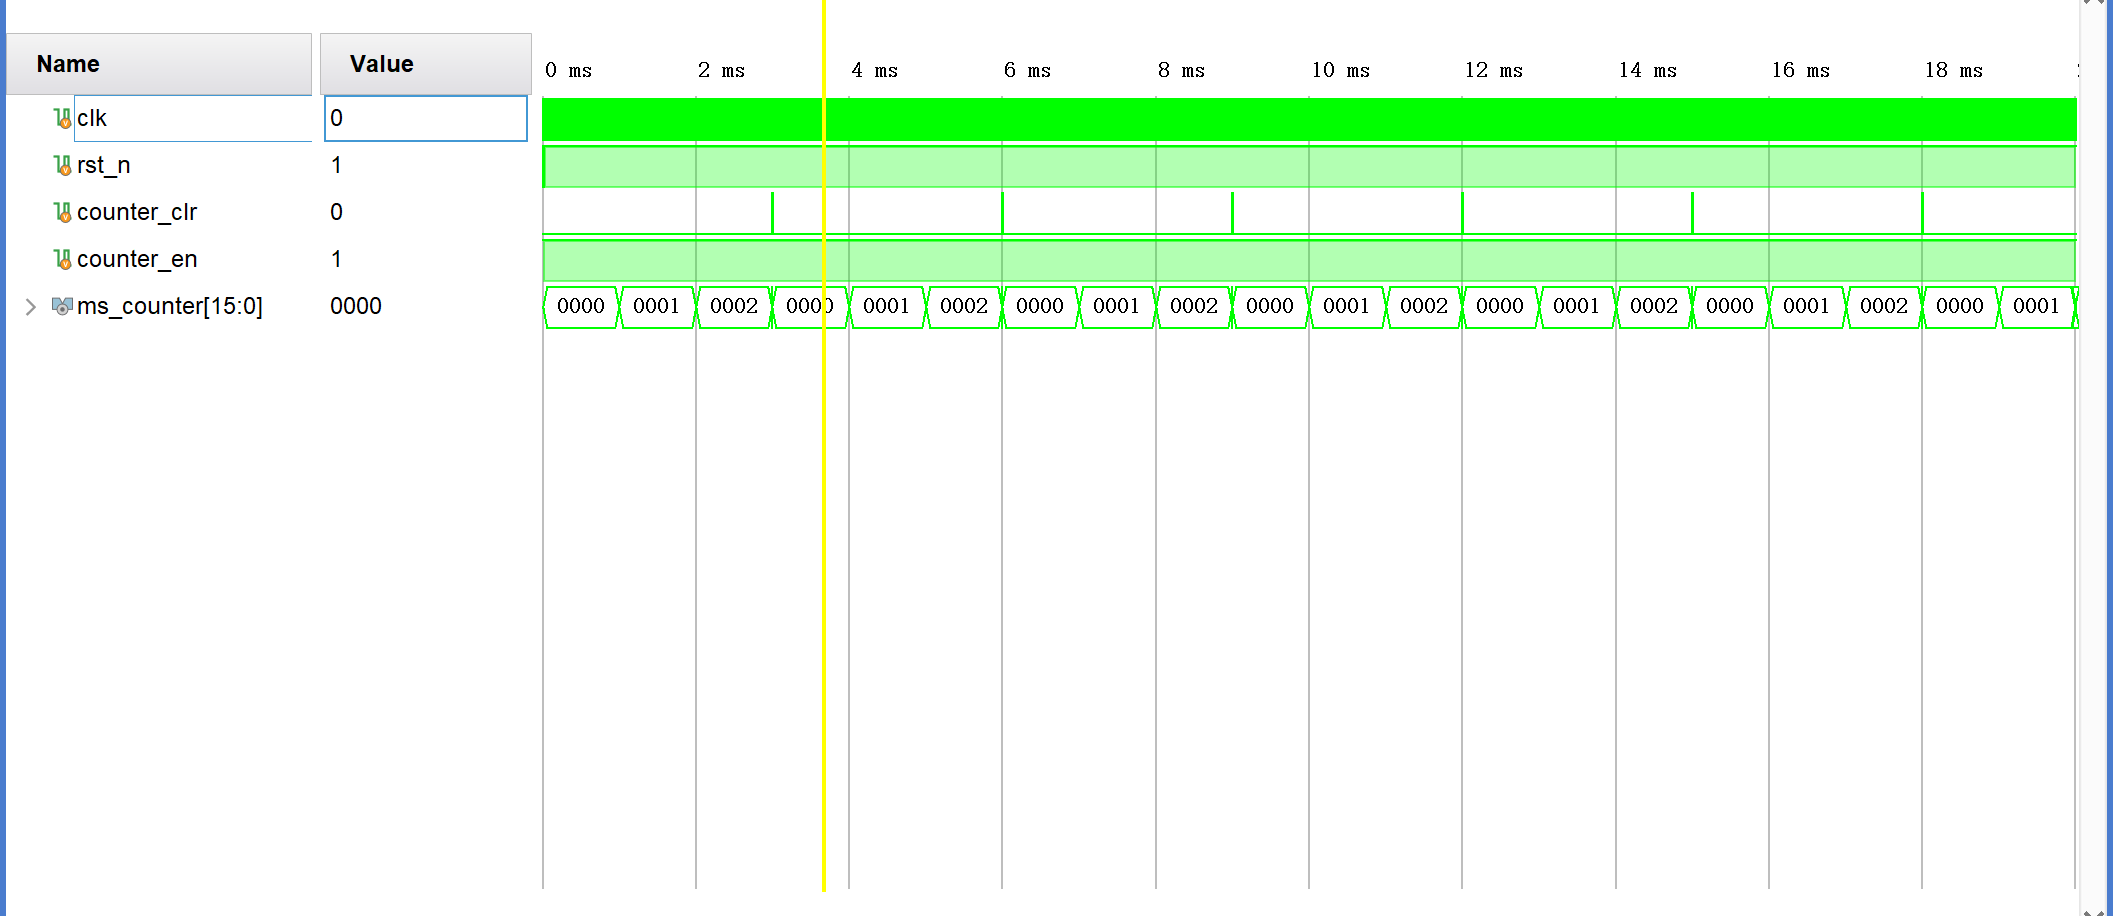
\includegraphics[width=0.92\textwidth]{fig/mstb.png}
  \caption{毫秒计数模块仿真波形}
  \label{fig:ms-counter-waveform}
\end{figure}
模块能正常工作。
\subsubsection{随机等待模块（\texttt{lfsr\_random\_service}）}
\paragraph{实现}
随机等待模块用于生成随机数，作为每轮测试开始后的随机等待时间。模块输入为系统时钟、复位和随机数请求信号 \texttt{req\_random}，输出为随机数有效信号 \texttt{random\_valid} 以及映射后的等待时间 \texttt{random\_delay\_ms}。

本设计采用 16 位 Fibonacci 结构 LFSR 产生伪随机序列，若第 $k$ 拍寄存器状态为 $s_k$，则下一拍状态为
\[
s_{k+1}=\{s_k[14:0],\; s_k[15]\oplus s_k[13]\oplus s_k[12]\oplus s_k[10]\}.
\]
为降低固定种子可预测性，模块引入 32 位自由运行计数器 $c_k$ 并做折叠扰动：
\[
e_k=c_k[15:0]\oplus c_k[31:16]\oplus \{c_k[7:0],\,c_k[15:8]\},
\]

\[
c_{k+1}=c_k+1 \pmod{2^{32}},
\]
而最终给出的随机数为
\[
r_k=s_{k+1}\oplus e_k,
\]


在收到 \texttt{req\_random} 上升沿时，输出等待时间按下式映射到$[\texttt{WAIT\_MIN\_MS},\texttt{WAIT\_MAX\_MS}]$ 区间内：
\[
\texttt{random\_delay\_ms}=\texttt{WAIT\_MIN\_MS}+\bigl(r_k\bmod(\texttt{WAIT\_MAX\_MS}-\texttt{WAIT\_MIN\_MS}+1)\bigr),
\]


\paragraph{仿真}
随机等待模块仿真中每隔 $10\,\mu s$ 给出一次 \texttt{req\_random} 请求脉冲。波形显示 \texttt{random\_valid} 能够在请求后给出有效响应，\texttt{random\_delay\_ms} 随请求更新且处于设定范围内，模块工作正常。

\begin{figure}[H]
  \centering
  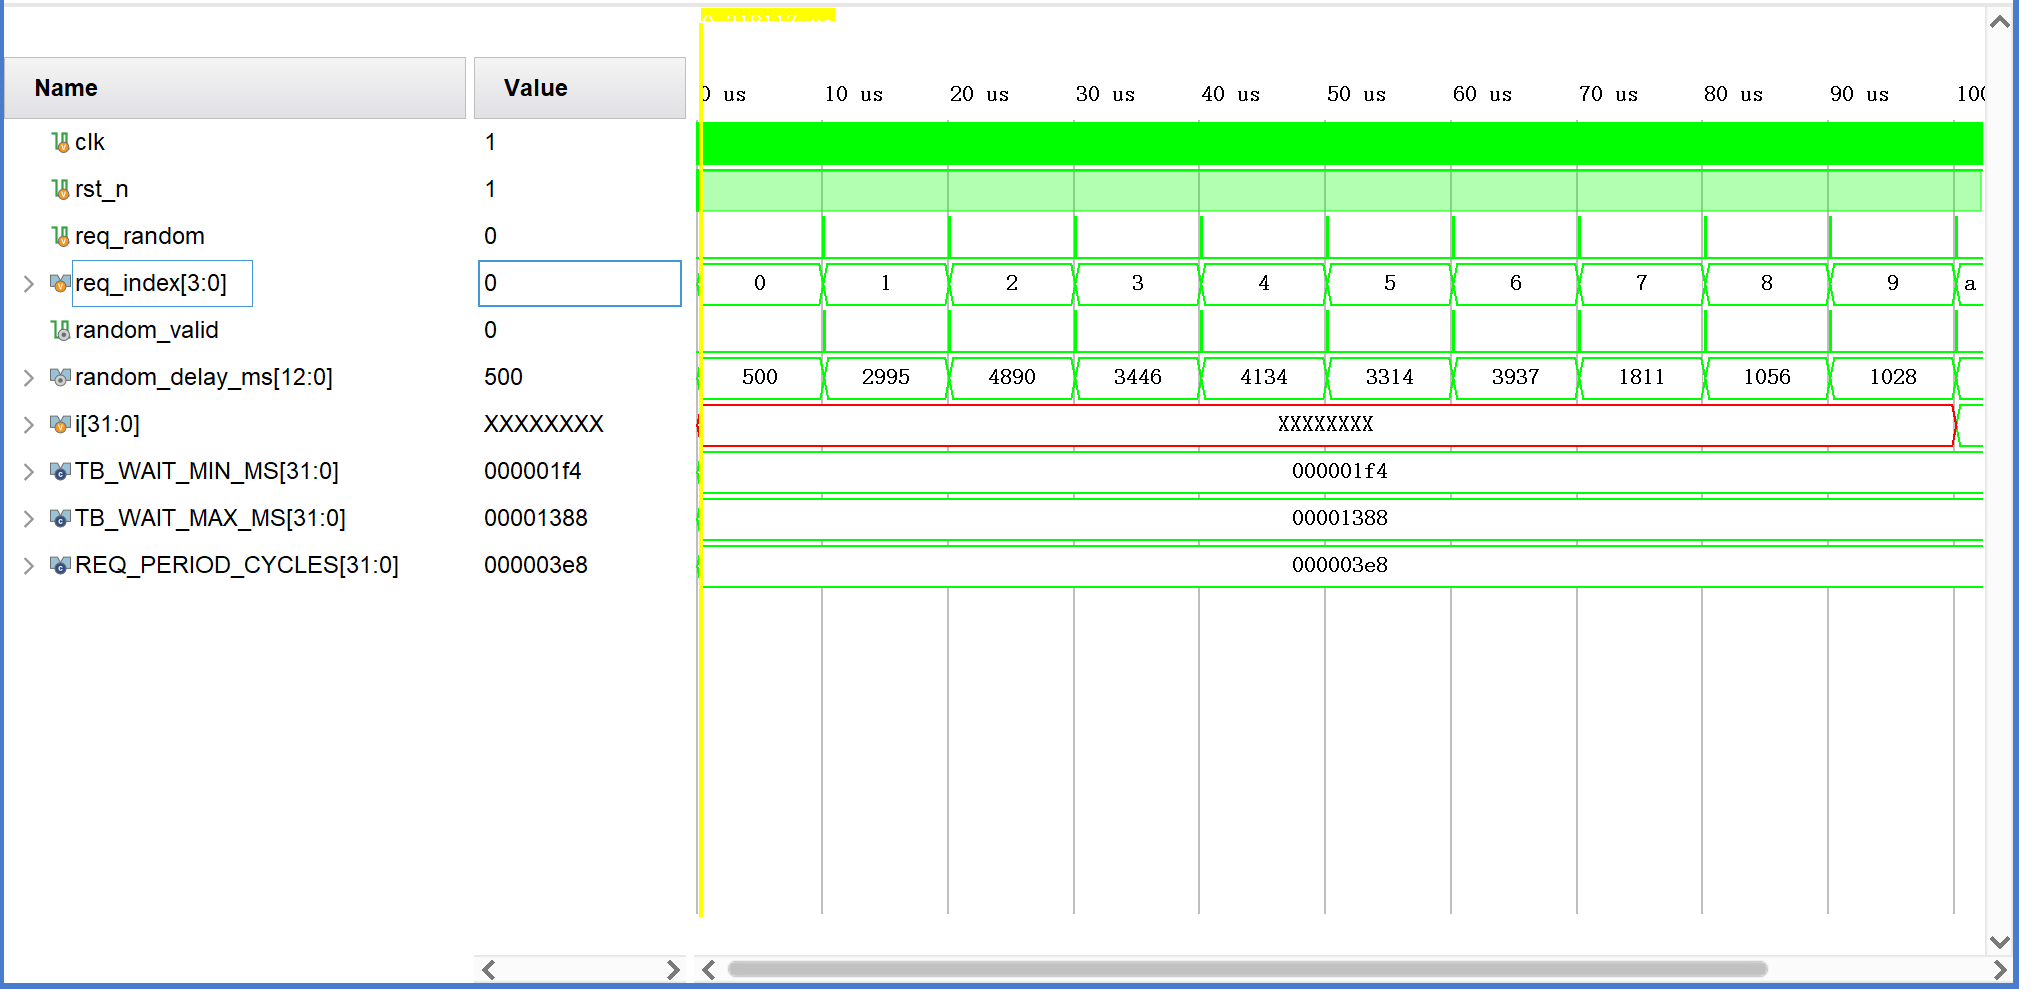
\includegraphics[width=0.92\textwidth]{fig/randomtb.png}
  \caption{随机等待模块仿真波形}
  \label{fig:random-service-waveform}
\end{figure}

\subsubsection{历史平均模块（\texttt{score\_history\_avg}）}
\paragraph{实现}
历史平均模块用于保存最近三次有效反应成绩，并计算其平均值供 AVG 状态显示。模块输入包括写入有效信号 \texttt{push\_valid} 和本次有效反应时间 \texttt{push\_time\_ms}，输出包括平均值有效标志 \texttt{avg\_valid} 和平均反应时间 \texttt{avg\_time\_ms}。

该模块采用滚动窗口结构保存历史成绩。当 \texttt{push\_valid} 有效时，模块将本次成绩写入历史队列；若已有三次成绩，则新成绩写入后会淘汰最早一次成绩。只有控制器判定为有效反应并产生 \texttt{score\_push\_valid} 时，历史模块才会更新，因此提前按键、过短反应和超时失败等无效结果不会进入历史平均统计。如果没有历史数据，会输出0000，如果有效历史数据少于3个，会根据保存的测试次数取平均。

\paragraph{仿真}
该模块仿真时依次输入多组有效成绩，观察平均值是否随样本数量正确变化；随后输入第四组有效成绩，观察最旧数据是否被替换；随后是失败场景，历史模块输入端保持 \texttt{push\_valid}=0，波形上可看到历史平均值不会因失败结果而改变。

\begin{figure}[H]
  \centering
  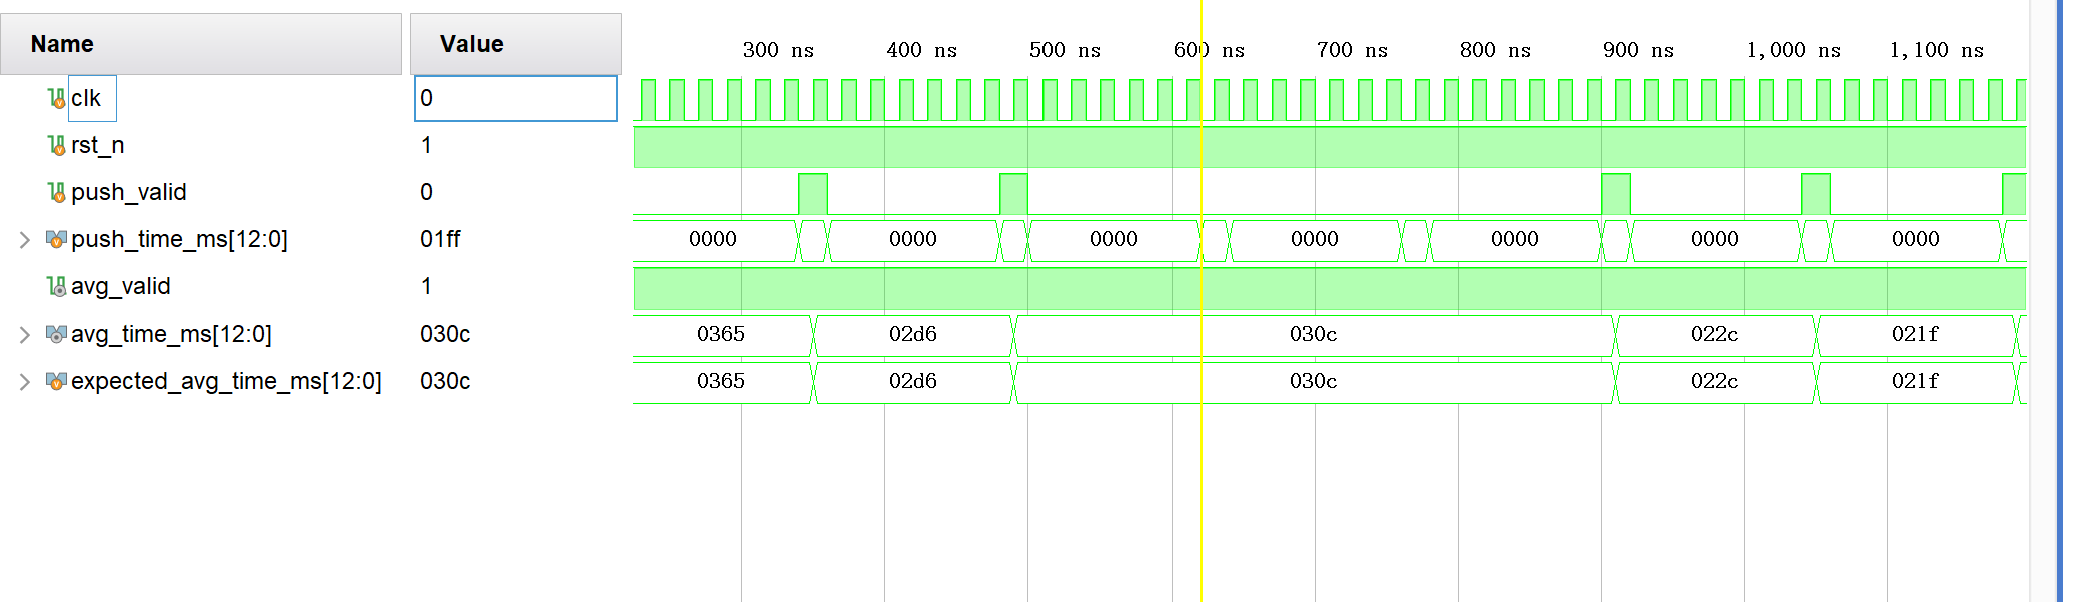
\includegraphics[width=0.92\textwidth]{fig/histtb.png}
  \caption{历史平均模块仿真波形}
  \label{fig:history-avg-waveform}
\end{figure}

\subsubsection{控制器模块（\texttt{reaction\_controller}）}
\paragraph{实现}
控制器模块是本系统的状态机核心，负责根据 START、REACT 按键脉冲、随机等待完成标志和毫秒计数值决定系统状态转移，并产生各子模块所需的控制信号。其主要输出包括随机数请求 \texttt{req\_random}、计数器清零 \texttt{counter\_clr}、计数器使能 \texttt{counter\_en}、成绩写入有效 \texttt{score\_push\_valid}、失败码 \texttt{fail\_code} 和当前反应时间 \texttt{reaction\_time\_ms}。

控制器状态机包含 \texttt{IDLE}、\texttt{PREPARE}、\texttt{WAIT}、\texttt{REACT}、\texttt{FINISH}、\texttt{AVG} 和 \texttt{FAIL} 七个状态。用户按下 START 后，控制器进入 \texttt{PREPARE} 并请求随机等待时间；随机数有效后进入 \texttt{WAIT}，此时计数器给ms时钟发送清零信号并监听其时钟值。若等待阶段提前按下 REACT，则进入失败状态；若等待时间达到随机目标值，则进入 \texttt{REACT} 并重新发送ms时钟清零，监听ms时钟获得反应时间。用户在有效时间范围内按下 REACT 时进入 \texttt{FINISH} 并写入成绩；若反应时间小于最小阈值或超过最大阈值，则进入 \texttt{FAIL}。

\paragraph{仿真}
控制器仿真采用固定输入激励观察状态转移波形。测试平台中将随机等待时间固定为 $1234\,\mathrm{ms}$，在 \texttt{WAIT} 阶段手动使 \texttt{ms\_counter} 每个时钟周期增加 $10\,\mathrm{ms}$，从而压缩仿真时间并清晰展示状态变化。仿真覆盖正常流程、等待阶段提前按键、小于最小反应时间按键以及超过最大反应时间按键四种情况。波形中重点观察 \texttt{state}、\texttt{start\_pulse}、\texttt{react\_pulse}、\texttt{ms\_counter}、\texttt{counter\_clr}、\texttt{counter\_en}、\texttt{fail\_code} 和 \texttt{score\_push\_valid} 的对应关系。

\begin{figure}[H]
  \centering
  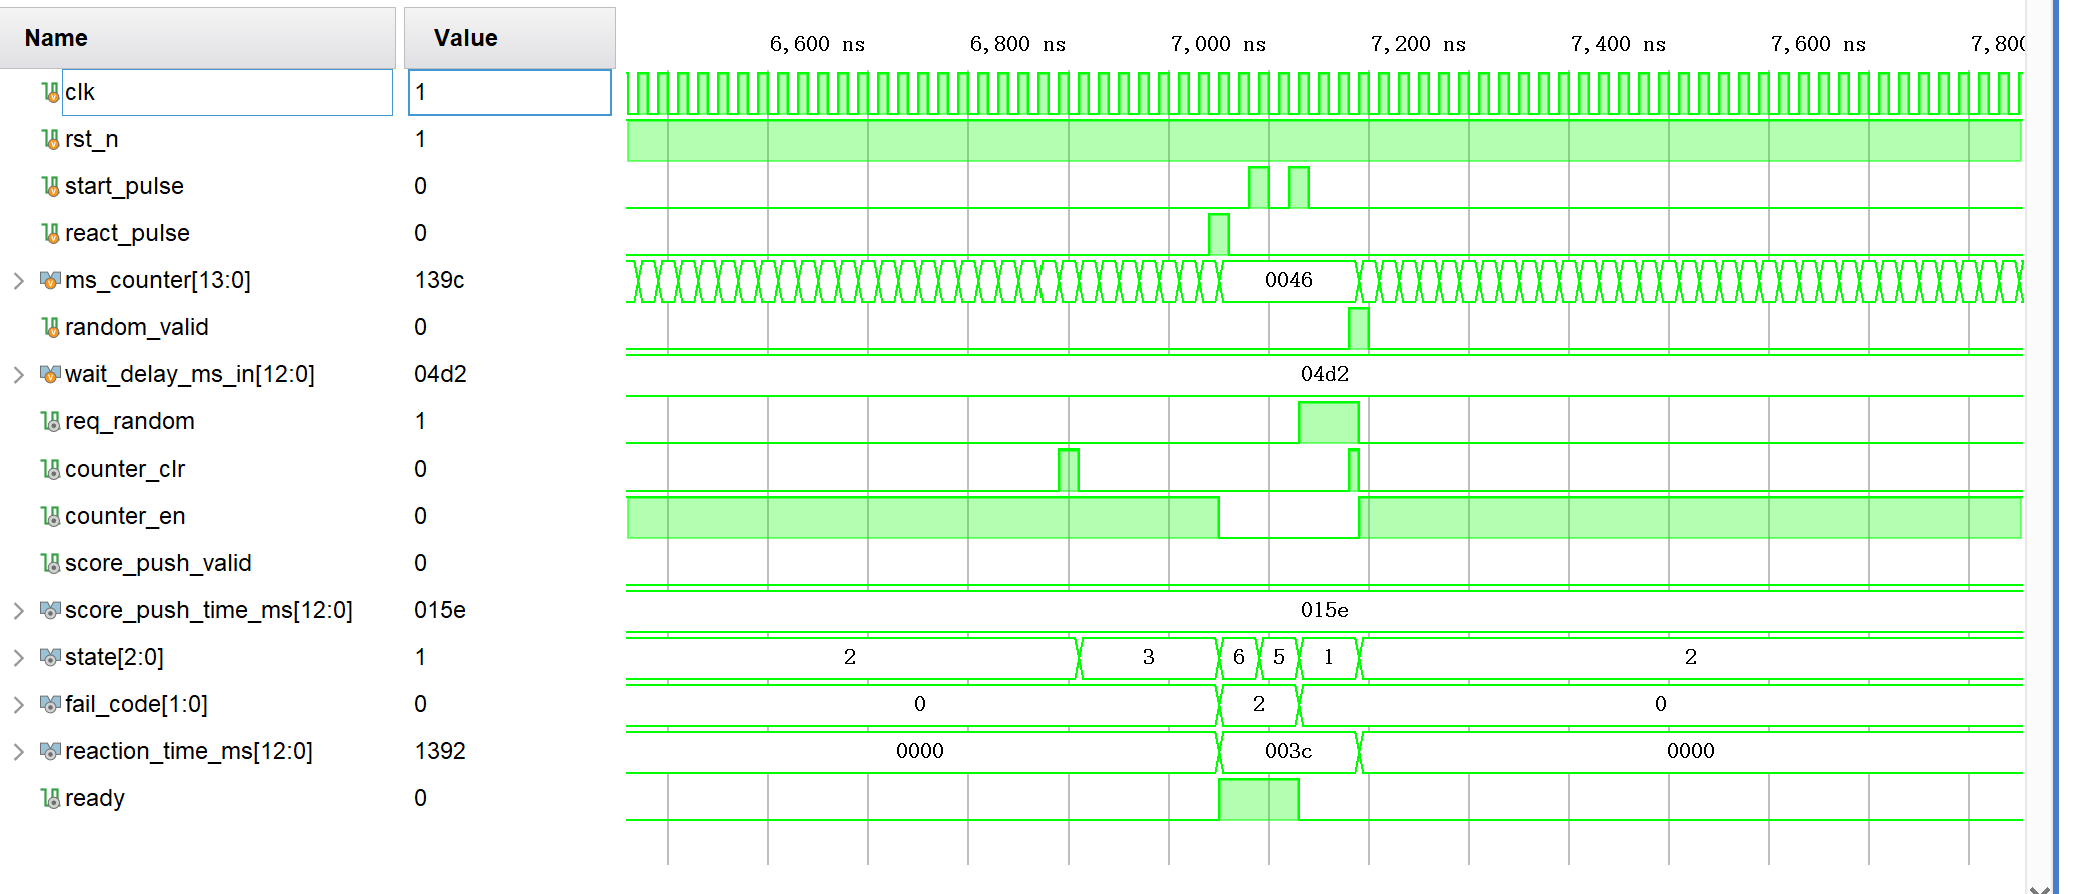
\includegraphics[width=0.92\textwidth]{fig/ctrltb.png}
  \caption{控制器模块仿真波形}
  \label{fig:controller-waveform}
\end{figure}

\subsubsection{按键去抖模块（\texttt{button\_debounce\_pulse}）}
\paragraph{实现}
按键去抖模块用于将板上机械按键输入转换为稳定的单周期控制脉冲。

\texttt{button\_debounce\_pulse} 模块用于处理机械按键抖动。原始按键信号首先经过同步寄存器进入系统时钟域，随后通过稳定计数判断按键电平是否已经保持足够长时间。当检测到一次稳定按下时，模块输出单周期 \texttt{btn\_press\_pulse}，供控制器作为 START 或 REACT 事件使用。

\paragraph{仿真}
该模块仿真时通过构造抖动按键输入，观察只有稳定按下后才产生一个单周期脉冲。

\begin{figure}[H]
  \centering
  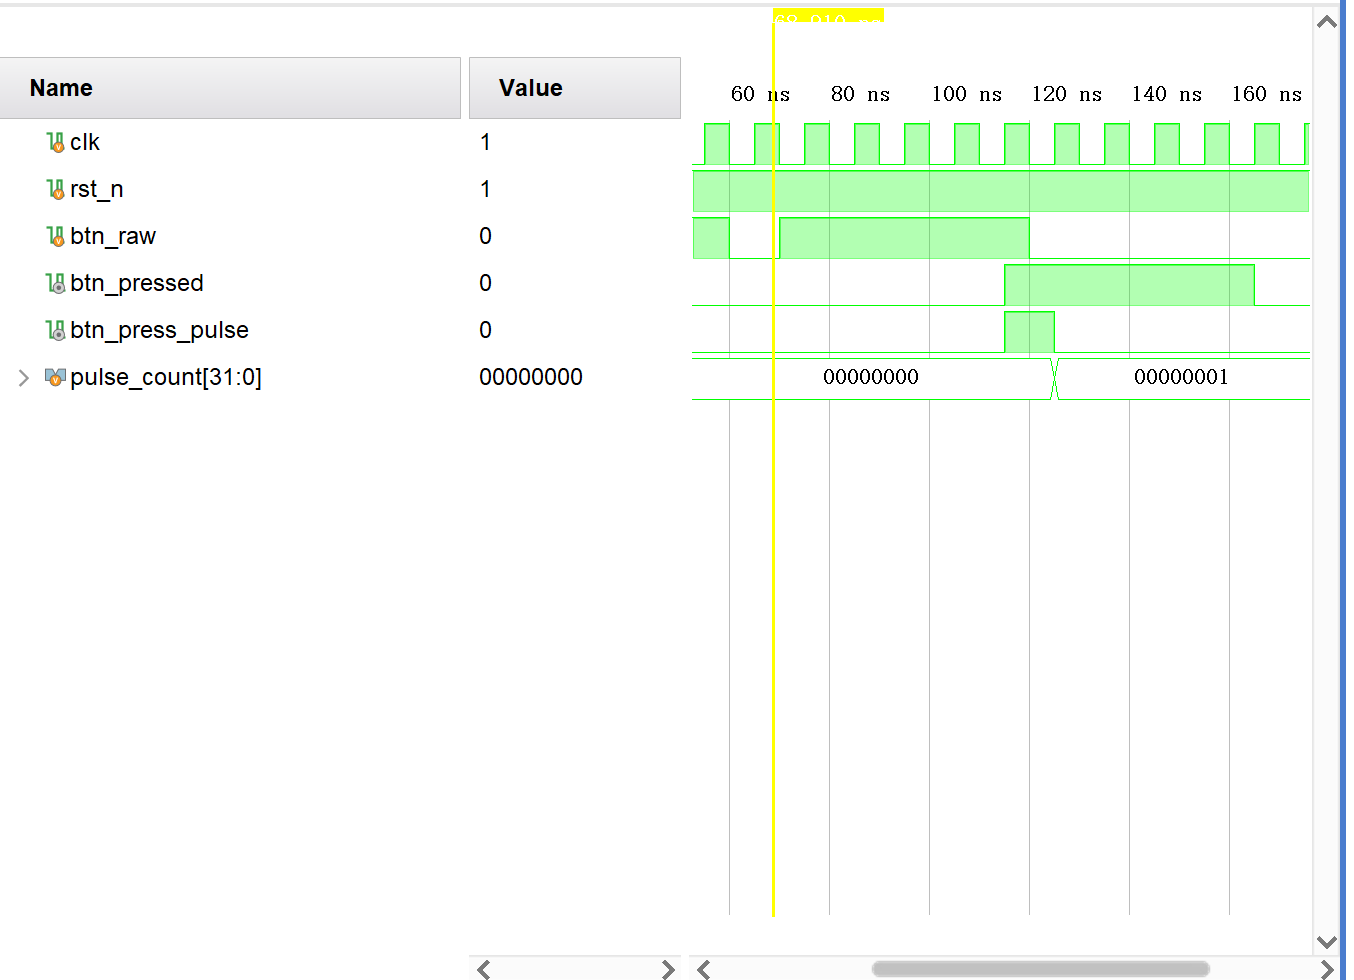
\includegraphics[width=0.92\textwidth]{fig/debuncetb.png}
  \caption{按键去抖模块仿真波形}
  \label{fig:debounce-waveform}
\end{figure}

\subsubsection{数码管显示模块（\texttt{seg7\_display\_driver}）}
\paragraph{实现}
\texttt{seg7\_display\_driver} 模块根据核心模块向外广播的当前状态决定四位八段数码管的段选与位选信号生成方式。在 \texttt{IDLE} 状态显示 \texttt{0000}；在 \texttt{PREPARE} 和 \texttt{WAIT} 状态显示 \texttt{----}；在 \texttt{REACT} 状态显示 \texttt{1111} 作为反应提示；在 \texttt{FINISH} 状态显示本次反应时间；在 \texttt{AVG} 状态显示最近三次有效成绩平均值；在 \texttt{FAIL} 状态显示 \texttt{FAIL}。对于数值或单词显示，模块先将二进制时间值拆分为十进制千、百、十、个位，再分别查表生成段码，对每个数位进行扫描。

\paragraph{仿真}
显示模块仿真时依次切换各个状态，观察段选信号 \texttt{seg\_a}--\texttt{seg\_dp} 与位选信号 \texttt{dig1}--\texttt{dig4} 的输出波形是否符合状态分类。

\begin{figure}[H]
  \centering
  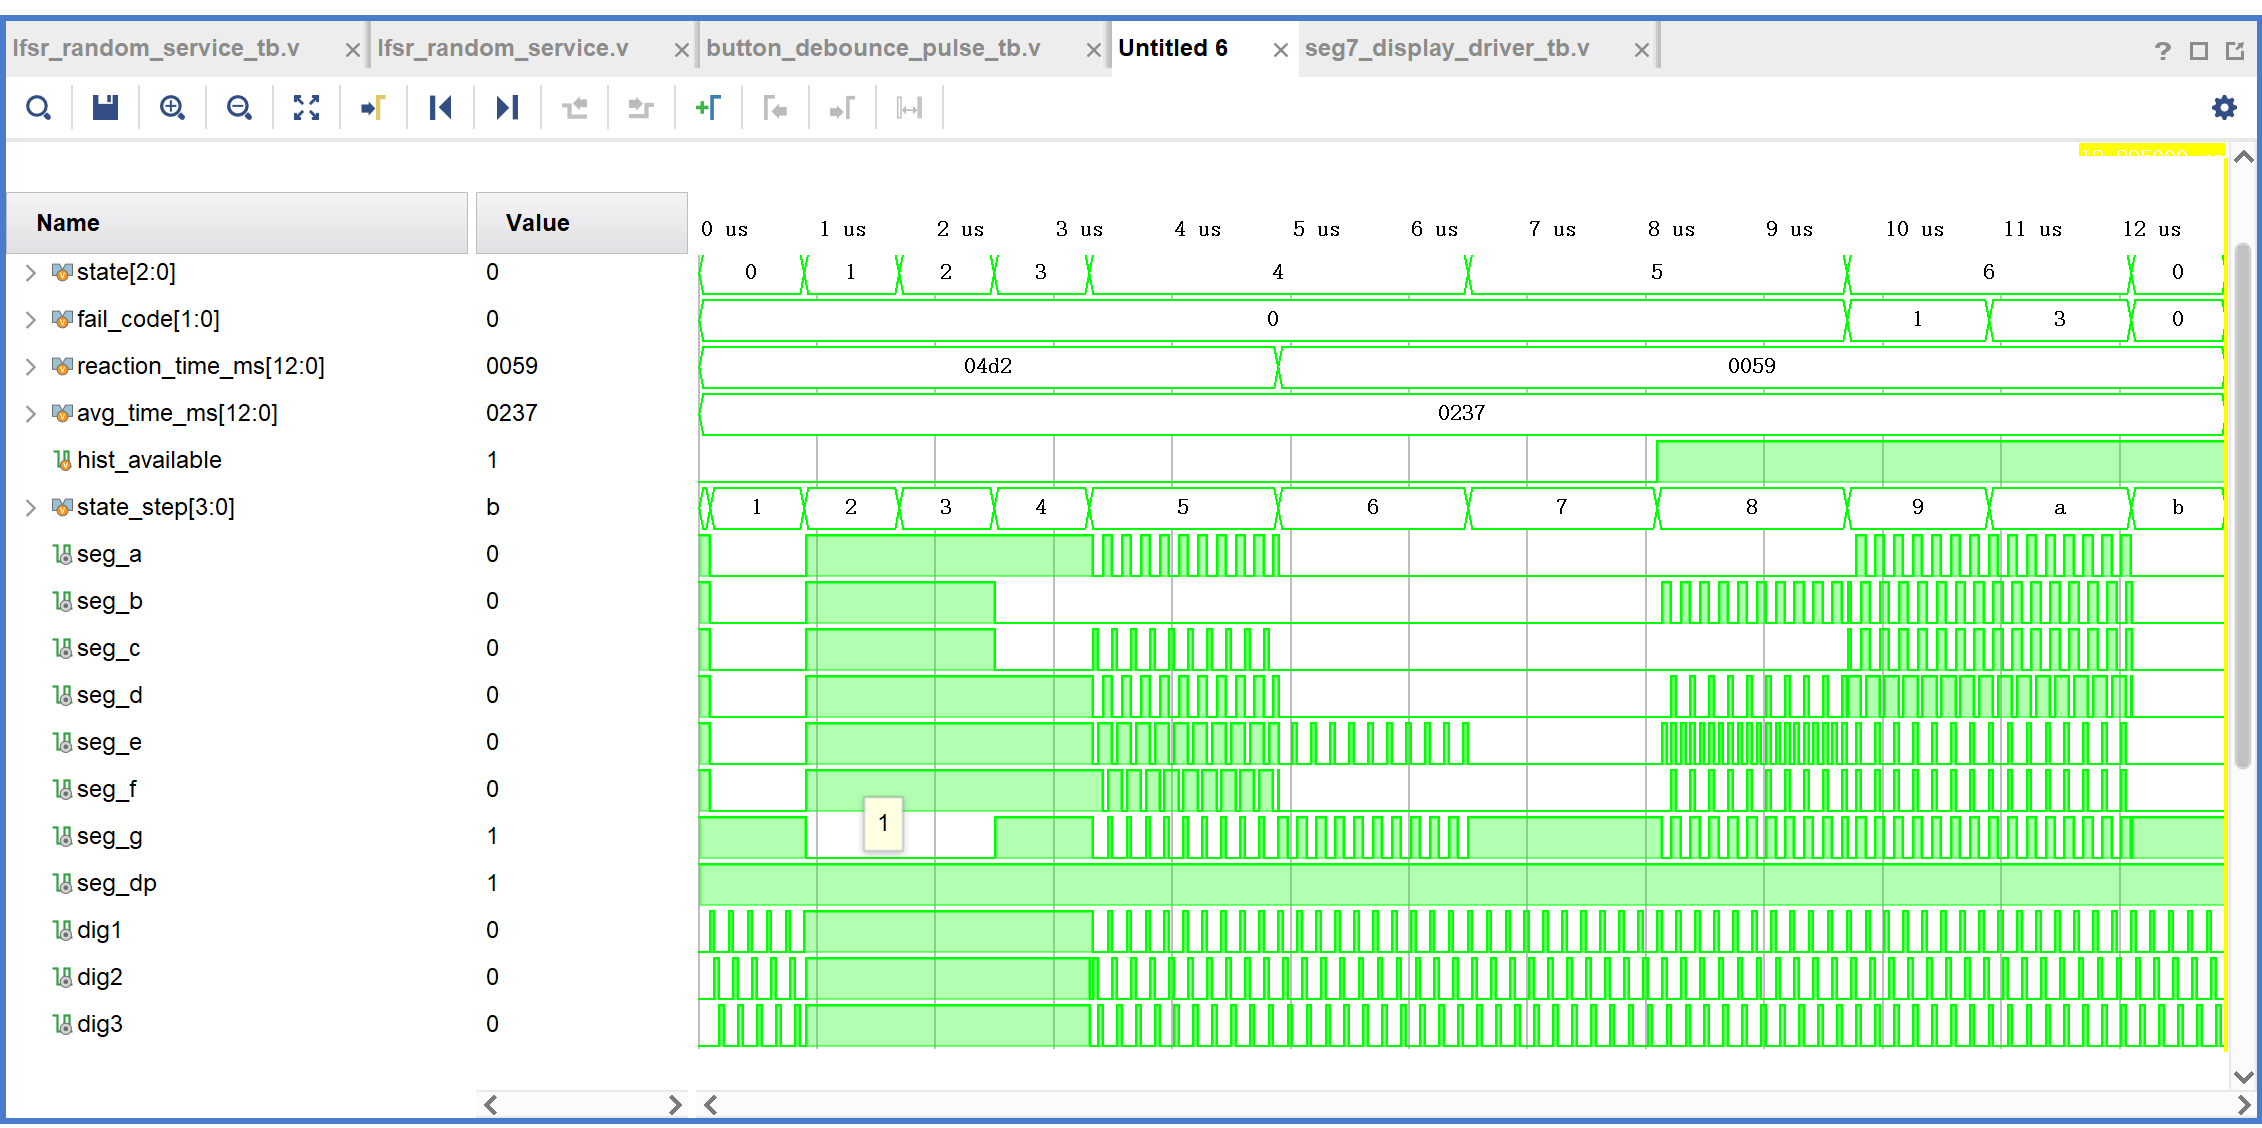
\includegraphics[width=0.92\textwidth]{fig/ledtb.png}
  \caption{数码管显示模块仿真波形}
  \label{fig:seg7-waveform}
\end{figure}

\subsubsection{蜂鸣器模块（\texttt{buzzer\_driver}）}
\paragraph{实现}
\texttt{buzzer\_driver} 模块用于提供声音提示。只要 \texttt{state} 与上一拍不同，就触发一次固定时长的短促蜂鸣。

\paragraph{仿真}
仿真时通过依次切换状态观察 \texttt{buzzer}，确认每次状态跳变均产生相同的短时提示波形。

\begin{figure}[H]
  \centering
  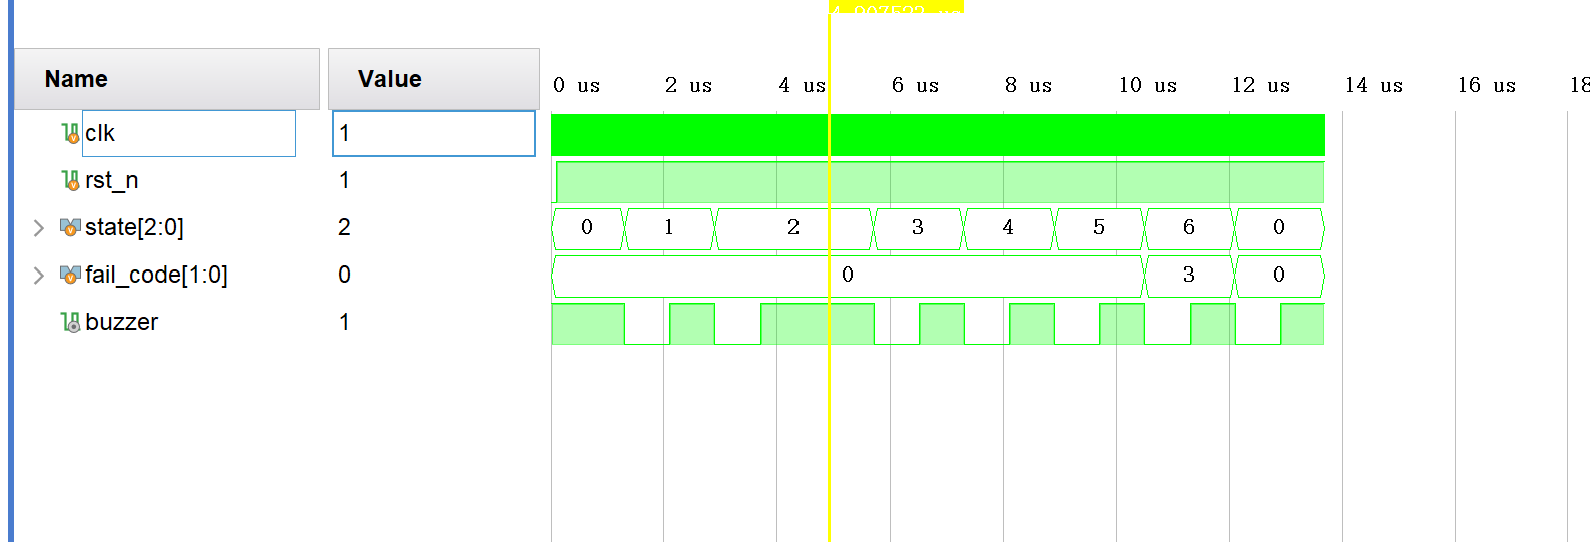
\includegraphics[width=0.92\textwidth]{fig/beep.png}
  \caption{蜂鸣器模块仿真波形}
  \label{fig:buzzer-waveform}
\end{figure}

\subsection{综合与实现}
\subsection{综合与实现结果}

本设计在 Vivado 2019.1 中完成综合、布局布线和 bitstream 生成，目标器件为 \texttt{xc7z020clg484-2}。实现结果主要来自 Vivado 在实现阶段生成的资源利用率报告、布局布线后时序报告和功耗估计报告。

\subsubsection{综合后资源利用率}

\begin{table}[H]
  \centering
  \caption{综合后资源利用率（synth\_1）}
  \label{tab:synth-utilization}
  \begin{tabular}{c|r|r|r}
    \hline
    Type & Used & Available & Utilisation \\
    \hline
    Slice LUTs & 802 & 53200 & 1.51\% \\
    Slice Registers & 430 & 106400 & 0.40\% \\
    Block RAM Tile & 0 & 140 & 0.00\% \\
    DSPs & 0 & 220 & 0.00\% \\
    Bonded IOB & 17 & 200 & 8.50\% \\
    BUFGCTRL & 1 & 32 & 3.13\% \\
    MMCME2\_ADV & 0 & 4 & 0.00\% \\
    PLLE2\_ADV & 0 & 4 & 0.00\% \\
    \hline
  \end{tabular}
\end{table}

\subsubsection{实现后资源利用率}

\begin{table}[H]
  \centering
  \caption{实现后资源利用率（impl\_1）}
  \label{tab:implementation-utilization}
  \begin{tabular}{c|r|r|r}
    \hline
    Type & Used & Available & Utilisation \\
    \hline
    Slice LUTs & 803 & 53200 & 1.51\% \\
    Slice Registers & 430 & 106400 & 0.40\% \\
    Block RAM Tile & 0 & 140 & 0.00\% \\
    DSPs & 0 & 220 & 0.00\% \\
    Bonded IOB & 17 & 200 & 8.50\% \\
    BUFGCTRL & 1 & 32 & 3.13\% \\
    MMCME2\_ADV & 0 & 4 & 0.00\% \\
    PLLE2\_ADV & 0 & 4 & 0.00\% \\
    \hline
  \end{tabular}
\end{table}

由表~\ref{tab:synth-utilization} 与表~\ref{tab:implementation-utilization} 可见，综合与实现阶段资源结果基本一致，系统主要消耗少量 LUT、触发器和 I/O 资源，未使用 Block RAM 与 DSP，整体资源占用较低。

\subsubsection{时序结果}

\begin{table}[H]
  \centering
  \caption{布局布线后时序结果}
  \label{tab:implementation-timing}
  \begin{tabular}{c|r}
    \hline
    Metric & Value \\
    \hline
    Worst Negative Slack (WNS) & 0.065 ns \\
    Total Negative Slack (TNS) & 0.000 ns \\
    TNS Failing Endpoints & 0 \\
    Worst Hold Slack (WHS) & 0.102 ns \\
    Total Hold Slack (THS) & 0.000 ns \\
    THS Failing Endpoints & 0 \\
    Worst Pulse Width Slack (WPWS) & 9.500 ns \\
    Total Pulse Width Slack (TPWS) & 0.000 ns \\
    \hline
  \end{tabular}
\end{table}

\begin{table}[H]
  \centering
  \caption{时钟约束摘要}
  \label{tab:implementation-clock-summary}
  \begin{tabular}{c|r|r}
    \hline
    Clock & Period & Frequency \\
    \hline
    \texttt{clk\_50m} & 20.000 ns & 50.000 MHz \\
    \hline
  \end{tabular}
\end{table}

Vivado 时序报告显示所有用户指定时序约束均已满足。根据主时钟周期和 WNS，可估算最大工作频率为
\[
F_{\max}=\frac{1000}{20.000-0.065}=50.16\,\mathrm{MHz}.
\]

\subsubsection{功耗结果}

\begin{table}[H]
  \centering
  \caption{布局布线后功耗估计}
  \label{tab:implementation-power}
  \begin{tabular}{c|r}
    \hline
    Metric & Value \\
    \hline
    Total On-Chip Power & 0.123 W \\
    Dynamic Power & 0.017 W \\
    Device Static Power & 0.106 W \\
    Junction Temperature & 26.4 $^\circ$C \\
    Confidence Level & Medium \\
    \hline
  \end{tabular}
\end{table}

综合以上结果，本设计在目标 FPGA 上能够满足 50 MHz 主时钟约束，资源占用和功耗均处于较低水平。

\subsection{静态时序结果分析}
根据实现后时序报告，主时钟 \texttt{clk\_50m} 约束满足，
关键指标为 \texttt{WNS>0}、\texttt{TNS=0}，说明设计满足 50 MHz 运行要求。

\section{FPGA 系统介绍、下载实现和调试，测试游戏过程}

本系统在 ZYNQ-Z7020 开发板上完成验证，START、REACT 和复位按键使用板上按键输入，数码管和蜂鸣器驱动电路外接在面包板上，使用开发板的GPIO pin连接，其中蜂鸣器通过三极管开关电路进行控制，是有源蜂鸣器，低有效。

\begin{figure}[H]
  \centering
  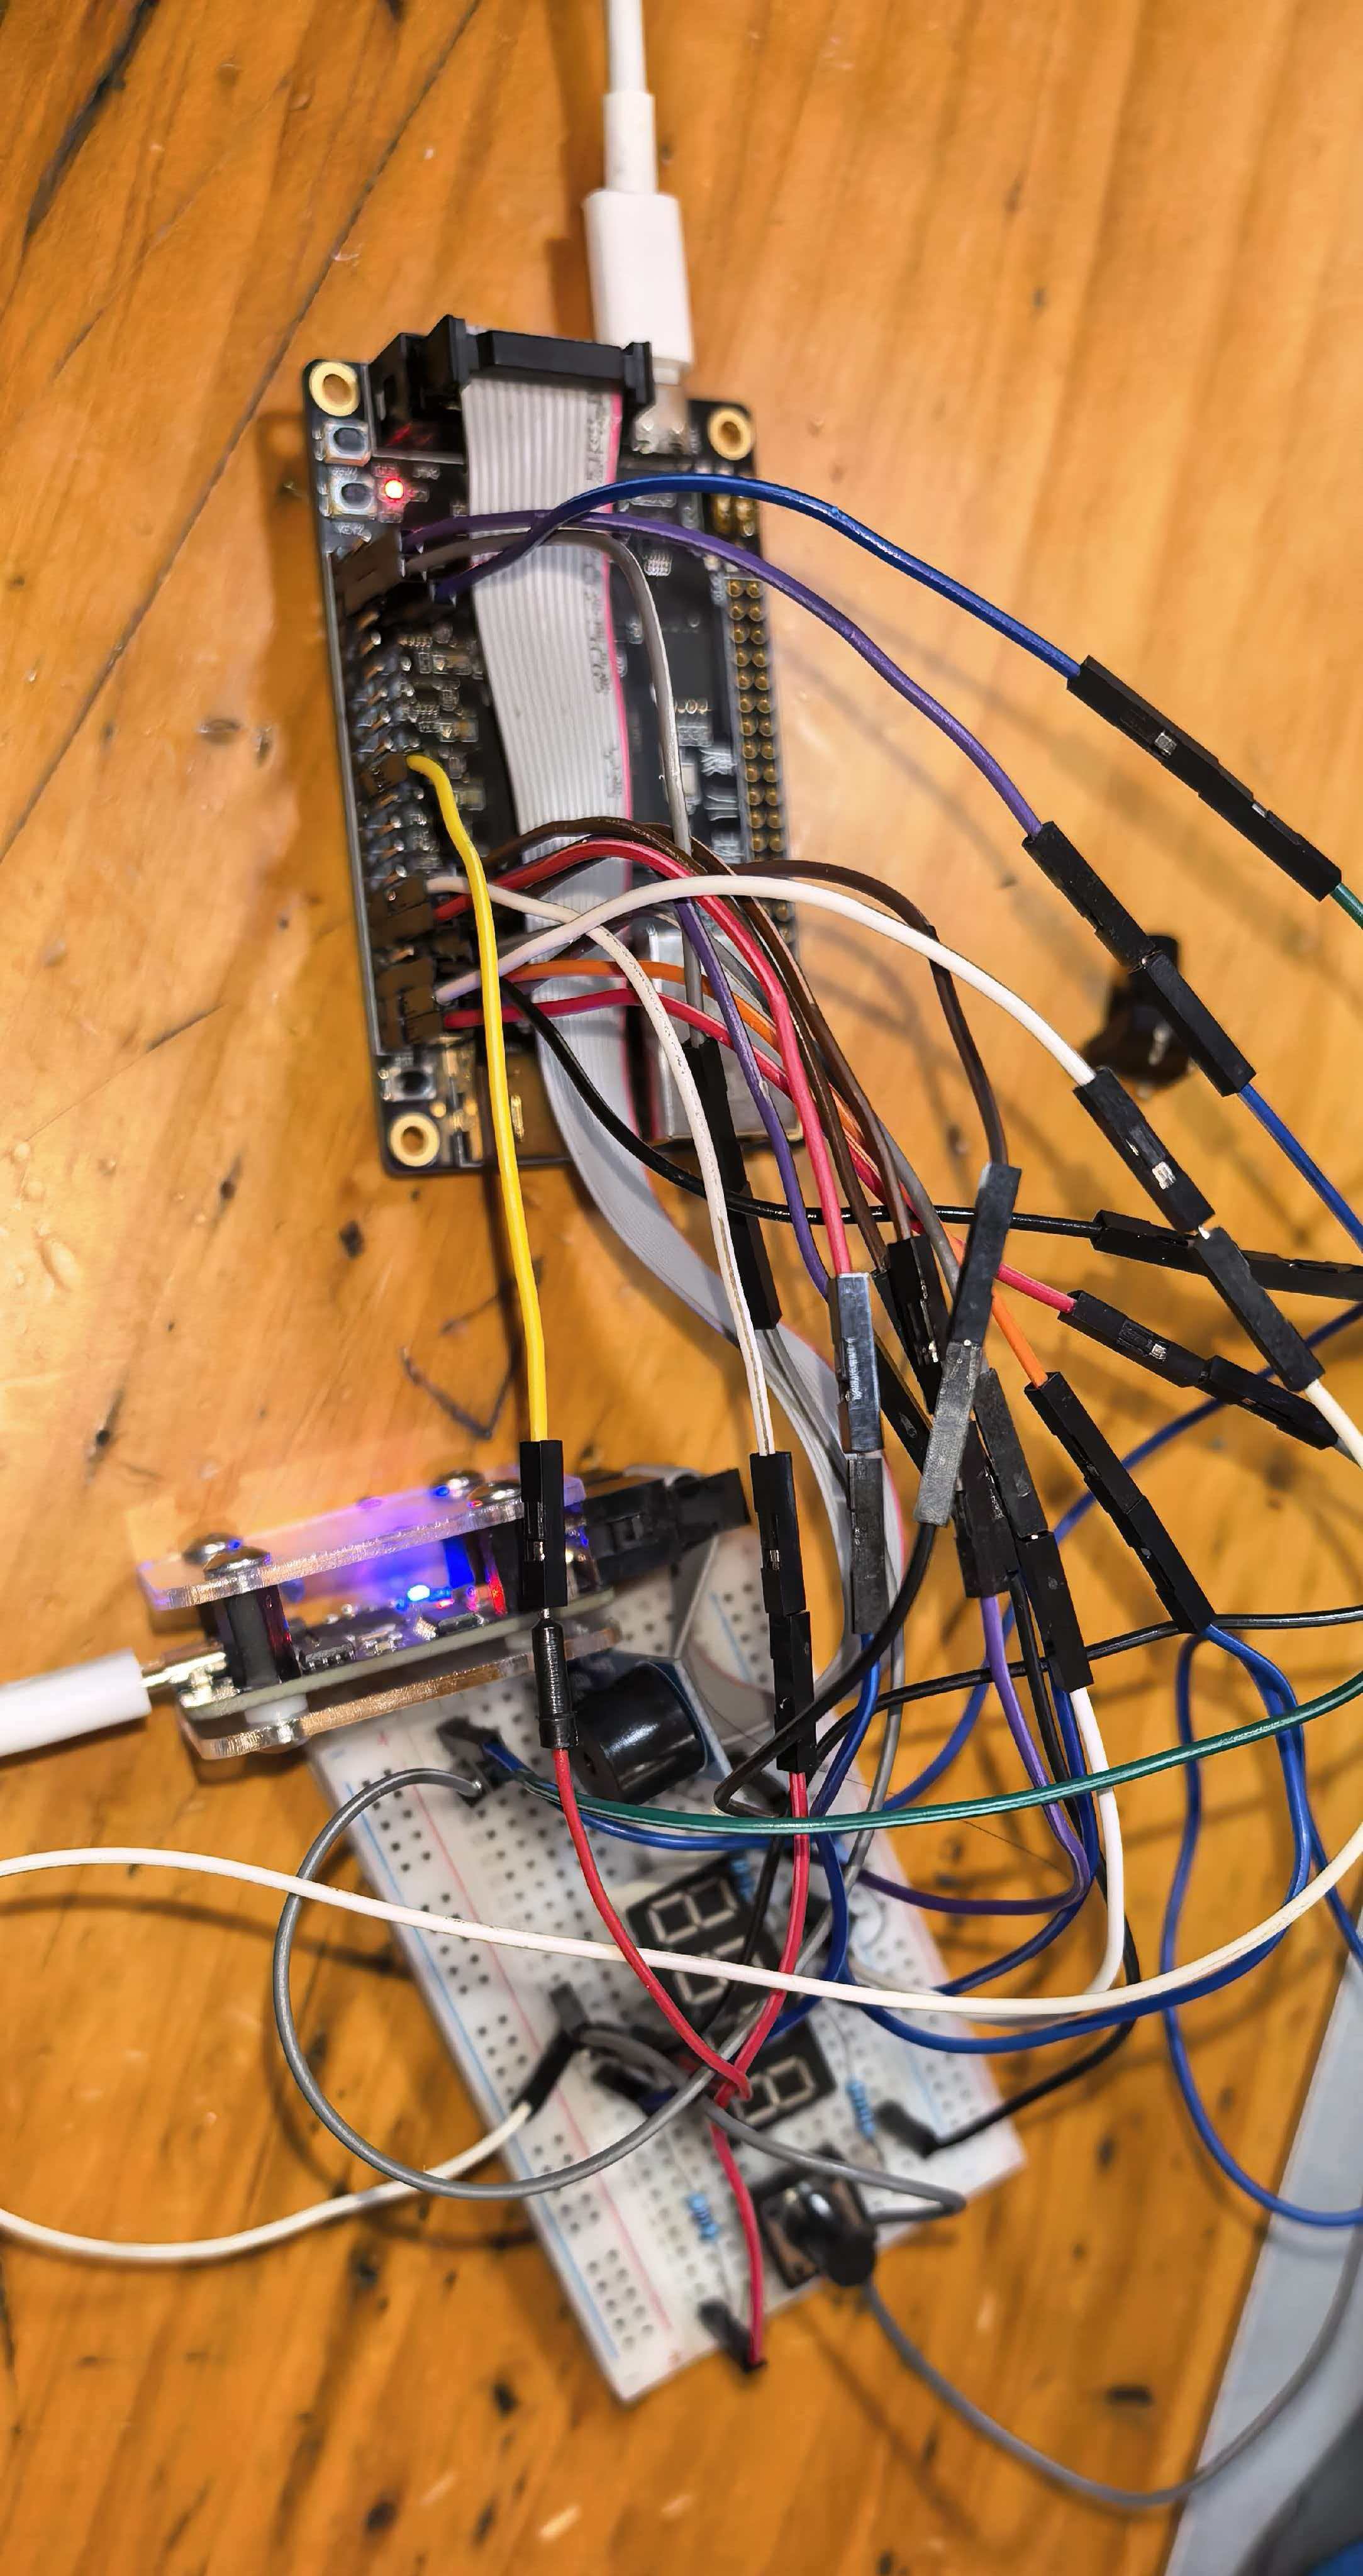
\includegraphics[width=0.68\textwidth,height=0.58\textheight,keepaspectratio]{fig/board.jpg}
  \caption{开发板与面包板外接电路实物图}
  \label{fig:board-external-circuit}
\end{figure}

\begin{figure}[H]
  \centering
  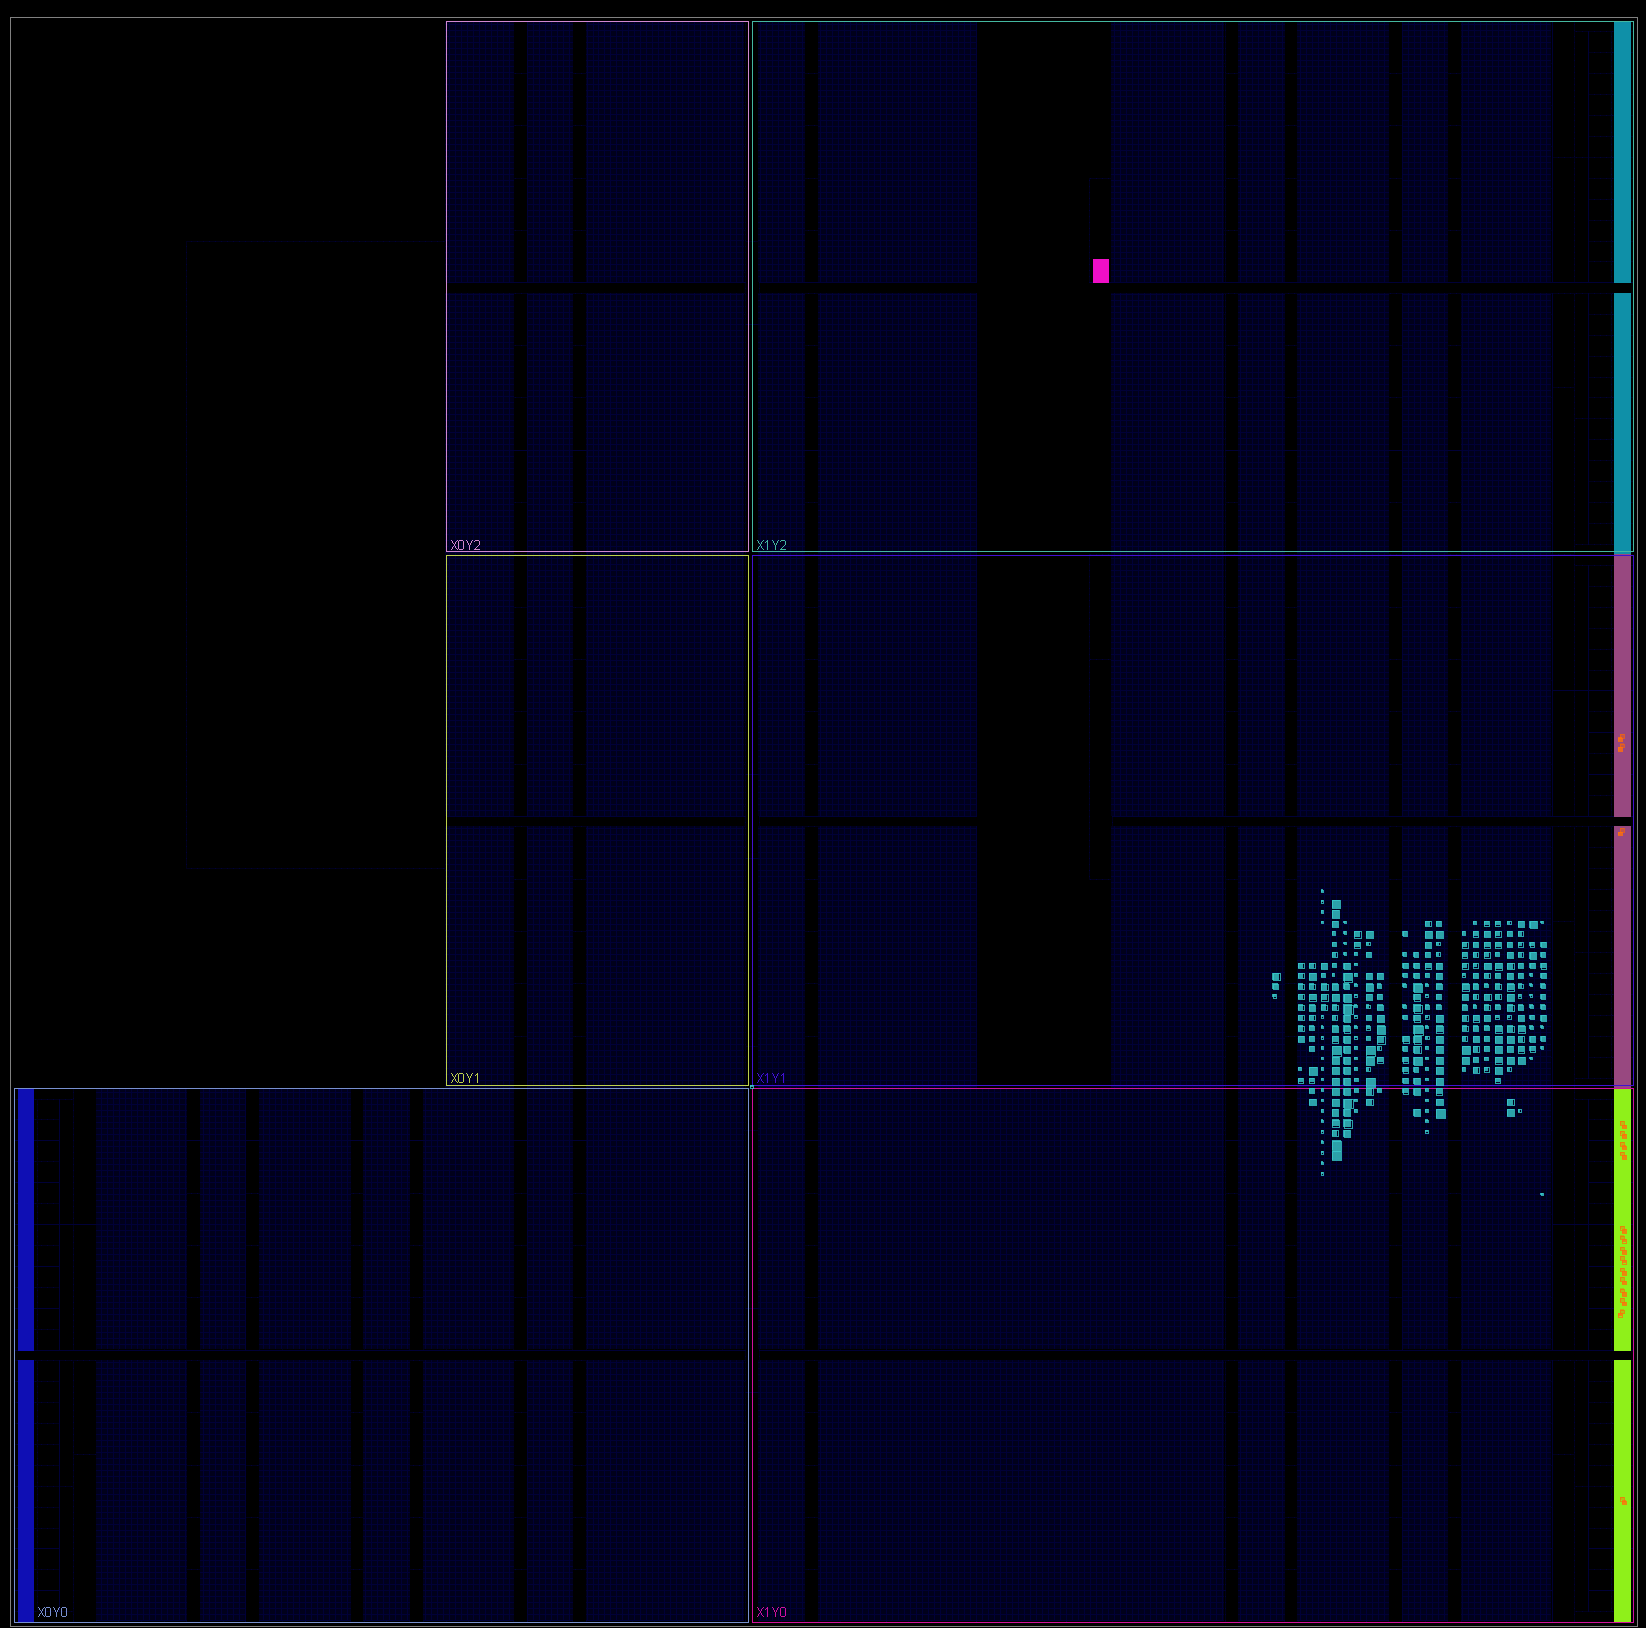
\includegraphics[width=0.92\textwidth]{fig/IMP.png}
  \caption{顶层连接实线部分的实现视图（IMP）}
  \label{fig:top-solid-impl-view}
\end{figure}

完成 synthesis 、implementation 和 bitstream 生成后，通过 usb连接线连接usb转jtag模块， 将设计下载到开发板。


上电后按 START 进入随机等待，待显示反应提示后按 REACT 记录反应时间。重复测试可观察 FAIL 判定与平均值显示逻辑。演示视频见文件夹内。

\section{设计总结}

本项目采用 Top-Down 的设计方法，从系统需求出发逐层细化到模块接口与 RTL 实现，完成了一个可在 FPGA 平台稳定运行的人体反应速度测试器。

在实现层面，系统以状态机为核心，结合随机等待、毫秒计时、成绩历史平均和数码管动态显示，形成了清晰的模块化架构。声音提示部分采用有源蜂鸣器驱动方案，通过低有效开关脉冲触发短鸣，不使用 PWM 波形合成，既符合外接三极管开关电路的硬件特性，也降低了控制逻辑复杂度。综合实现结果表明，本设计在 50 MHz 约束下时序收敛良好，资源占用和功耗均较低，满足课程要求并具备一定可复用性与扩展空间。

\section{个人体会}

通过本项目，我体会最深的有两点。第一，模块接口定义是整个设计过程中最需要前置思考的部分，尤其是脉冲信号应由发送端产生还是由接收端整形，不同选择会直接影响时序关系、模块耦合度和后续联调难度，因此必须在架构阶段明确约定并在各模块中保持一致。第二，每完成一个子模块都应及时进行仿真和波形核对，尽早发现并修正逻辑问题；这样在下板实现后若仍出现异常，可以将排查范围有效收敛到硬件连接、约束或器件特性，而不是进行盲目调试。

\section*{附：主要文件说明}
\begin{longtable}{p{0.34\textwidth} p{0.60\textwidth}}
\toprule
文件夹/路径 & GitHub 保留内容说明 \\
\midrule
\texttt{/}（仓库根目录） & 需求说明 \texttt{requirements.md}；演示视频文件（\texttt{演示.mp4}）以及构建脚本 \texttt{build\_bitstream.tcl}。 \\
\texttt{src/} & RTL 源码目录：\texttt{reaction\_system\_top.v}、\texttt{reaction\_core.v}、\texttt{reaction\_controller.v}、\texttt{lfsr\_random\_service.v}、\texttt{ms\_counter\_service.v}、\texttt{score\_history\_avg.v}、\texttt{seg7\_display\_driver.v}、\texttt{buzzer\_driver.v}、\texttt{button\_debounce\_pulse.v}。 \\
\texttt{sim/} & 仿真测试目录 \texttt{*\_tb.v}，用于功能验证与波形检查。 \\
\texttt{xdc/} & 约束目录 \texttt{reaction\_system\_gpio1.xdc}。 \\
\texttt{report/} & 课程报告与素材目录，主文档 \texttt{course\_report.tex}、分节 \texttt{section\_*.tex}、图像资源以及导出的 \texttt{course\_report.pdf}。 \\
\texttt{Vivado/} & Vivado 工程目录，保留工程文件与实现产物（如 \texttt{Vivado.xpr}、\texttt{Vivado.runs/}、\texttt{Vivado.hw/}），用于结果复现与工程追踪。 \\
\bottomrule
\end{longtable}

\end{document}
